\documentclass[a4paper]{article}

%% Language and font encodings
\usepackage[english]{babel}
\usepackage[utf8x]{inputenc}
% \usepackage[T1]{fontenc}

%% Sets page size and margins
\usepackage[a4paper,top=2.5cm,bottom=2cm,left=3cm,right=3cm,marginparwidth=1.75cm]{geometry}

%% Other packages
\usepackage{amsmath}
\usepackage{graphicx}
\usepackage[colorinlistoftodos]{todonotes}
\usepackage[colorlinks=true, allcolors=blue]{hyperref}
\usepackage{apacite}
\AtBeginDocument{\urlstyle{APACsame}}
\usepackage[section]{placeins}
\usepackage{adjustbox}
\usepackage{natbib}
\usepackage{booktabs}
\addto\captionsenglish{\renewcommand*\contentsname{Table of Contents}}

\title{\textbf{Patterns of Global and Regional Value Chain Participation in the EAC}}
% \author{Sebastian Krantz\footnote{Kiel Institute for the World Economy\\ \textit{Address:} Haus Welt-Club, Duesternbrooker Weg 148, D-24105 Kiel\\ \textit{E-mail:} sebastian.krantz@ifw-kiel.de}}
% \date{July 30, 2021}
\date{}

\begin{document}
\maketitle

%\vspace{1cm}

\begin{abstract}
Using global Multi-Region Input-Output (MRIO) data from 2005-2015, this paper empiri- 
cally investigates the extent and patterns by which East African Community (EAC) countries have integrated into Global Value Chains (GVCs) and Regional Value Chains (RVCs). Results imply that the foreign content of exports (I2E) and the share of exports being re-exported (E2R) are between 10\% and 20\% in most EAC countries. During 2005-2015, all EAC members apart from Kenya experienced a decline in E2R. Trade in intermediates with the rest of the world remains 12-14 times greater in value-added (VA) terms than inside the EAC. Kenya expanded its role as a regional supplier of manufactured inputs (higher E2R with EAC partners), and Uganda slightly increased its agricultural input to the Kenyan % and Rwandan 
food processing sector. Furthermore, a downstream shift is evident, by which more VA (both domestic and foreign) is used for the production of final goods while maintaining high levels of exports in primary agriculture and mining. Only Kenya was able to broadly maintain and improve its comparative advantage in manufacturing. Econometric analysis suggests that higher I2E and E2R shares increase GDP with an average elasticity of $\geq 0.25$ over 2 years. Estimates for manufacturing sectors were slightly higher at elasticities $\geq 0.3$ in response to E2R shifts. These results imply that policy measures to increase manufacturing competitiveness and promote more horizontal RVCs would benefit EAC economic growth in the medium run.  \\

\noindent \textbf{Keywords:} GVCs, EAC, regional integration, industrial development, comparative advantage\\
\textbf{JEL classification:} F14; F15; O11
\end{abstract}

% \tableofcontents
% \newpage
% \listoftables
% \listoffigures
% \newpage


\section{Introduction}

Global Value Chains (GVCs), referring to the quickly expanding internationalization of production networks, have become a central topic in trade and development policy. With the entry into force of AfCFTA in May 2019 and some progress towards its full enactment, the potential of a large common market in Africa for increased GVC-related trade, both within Africa and between Africa and the world, is of great interest to research and policy. To gauge the potential implications and distributional side-effects of AfCFTA for GVCs, it is, at least to some degree, instructive to study the effects of smaller efforts of regional integration and the creation of common markets in Africa, as has been the case in East Africa with the East African Community (EAC). \newline 

(Re-)founded in 2000 by Uganda, Kenya, and Tanzania as a body to facilitate regional coopera-
tion, the EAC quickly became a vehicle for economic integration. A customs union became operational in January 2005, with Kenya, the region's largest exporter, continuing to pay duties on some goods entering other countries on a declining scale until 2010 (EAC Customs Union Protocol, Article 11 and \citet{aloo2017free}). Rwanda and Burundi acceded in 2007, joining the customs union in 2009. The customs union expanded to a common market for goods, labor, and capital effective in 2010. In 2013, the Protocol for the Establishment of the EAC Monetary Union was signed, aiming for a monetary union within 10 years, subject to macro-fiscal convergence criteria. In 2016 the newly founded Republic of South Sudan joined the EAC, and the Democratic Republic of Congo joined in July 2022. Thus the EAC, particularly the years following the customs union in 2005 and the common market in 2010, provides a small case study in light of AfCFTA's broader aims. \newline 

While some work has been done on RVCs in East Africa within specific industries, such as Maize value chains studied by \citet{daly2016maize}, there has not yet been a detailed exposition of the GVC participation of East African Countries using comprehensive data sources such as Inter-Country Input-Output (ICIO) tables and databases. Some landmark studies have however been conducted regarding the GVC integration of Africa and developing countries more broadly. \newline

\citet{foster2015global} provide one of the first comprehensive analyses of GVCs in Africa, using the EORA 25 sector database over the periods from 2000-2011. They find that Africa as a region is more involved in GVCs than many other developing regions, but much of the GVC involvement of Africa is in upstream production and involves the supply of primary goods. Downstream involvement is relatively small and shows little improvement in the 1995-2011 period. GVC involvement is very heterogeneous across African countries, with some relatively successful countries heavily involved in (downstream) GVCs. At a sectoral level, \citet{foster2015global} find that manufacturing and high-tech sectors are typically not major contributors to African GVC participation. Inner-African GVCs are also small in most African countries, with several exceptions in southern Africa. The EU is the biggest GVC partner for Africa, with increasing shares of (South-)East Asia and other transition countries. \newline

Another broad analysis of GVC participation focusing on Africa, the Middle East, and Asia is provided by \citet{kowalski2015participation}\footnote{The authors conduct extensive econometric analysis using GVC indicators computed from OECD TiVA ICIOs for 57 countries in the years 1995, 2000, 2005, 2008, and 2008, WIOD ICIOs for 40 countries from 1995-2011, and EORA ICIOs for 186 countries from 1990-2011, as well as country-specific structural and policy indicators.}.
They find that structural factors, such as geographic proximity to manufacturing hubs in Europe, North America, and East Asia, domestic market size, and the level of development, are key determinants of GVC participation. In addition, trade and investment policy reforms (in particular low import tariffs and FDI openness), improvements in logistics and customs, intellectual property protection, infrastructure, and institutions can play a large role in promoting further engagement. %They state that very favorable policy environments in low-income countries can substitute to some extent for suboptimal structural factors. 
Developing countries reap important benefits from GVC participation through both forward and backward linkages, including enhanced productivity, export diversification, and sophistication. Analyzing export competitiveness in different regions, they find that Asia dominates more advanced products such as electronic equipment or motor vehicles, while African and Middle Eastern regions are competitive in agriculture, food processing, and less advanced manufacturing. While all regions have become more competitive, they find little signs for a trend towards industriali- 
zation and GVC-related trade in Africa. The survival rates of export relationships in Asia are also near twice that of African export relationships. \newline  % , which they attribute to stronger regional integration and learning by doing. \newline %In terms of global integration, they find that advanced economies are becoming less important as suppliers of inputs to developing regions and that trade in intermediates is increasing both between and within the South Asia, Middle-East, and Africa regions. Finally, they find that services trade also takes on an increasing role for GVCs in various developing regions. \newline 

A broader research-oriented perspective on GVCs is provided in \citet{Kummritz20162} and \citet{Kummritz20161}. \citet{Kummritz20162} examine patterns of GVC integration in low- and middle-income countries using the OECD TiVA database\footnote{Covering 61 countries and 34 industries for the years 1995, 2000, 2005, and 2008 to 2011.}. They find that, apart from agriculture, developing countries are typically located more downstream in the value chain, and export more final goods. High-income economies use GVCs to outsource low value-added (VA) downstream production stages and eventually reimport the final good. Over time, many developing economies have succeeded in moving up the value chain, and the general trend points to a more even distribution of VA across countries. South-East Asia has the highest levels of GVC integration. %, while Latin America and the Caribbean are more heterogenous with Chile and Costa Rica performing very well. 
In Africa, Tunisia has developed backward linkages into GVCs, especially with the EU. 
Overall, their findings suggest that low- and middle-income countries have become an integral part of GVCs, where the foreign content of global VA exports attributable to these countries has risen from 9\% in 1995 to 24\% in 2011, and the share in re-exported exports has increased from 9\% to 23\%. These countries are becoming drivers of GVC expansion and proceeding up the value chain to more upstream tasks, with beneficial effects for domestic industrialization. \newline

The main aim of this paper is to map the structure of regional and international production and exports in the EAC and to produce some first evidence of the potential benefits of GVC integration for East Africa at the aggregate and sector levels. A secondary aim, more difficult to substantiate empirically, is to gauge the potential effects of regional economic integration through a customs union (2005) and common market (2010) for GVC-related trade in and with the EAC. The analysis follows the seminal works of \citet{hummels2001nature}, \citet{koopman2014tracing}, \citet{wang2013quantifying}, as well as \citet{Kummritz20161} and \citet{Kummritz20162}\footnote{More sophisticated GVC decompositions or econometric approaches are considered infeasible in light of the low quality of the EORA ICIO tables for developing countries.}. 

\newpage

\section{Data}

Most GVC analysis uses Inter-Country Input-Output tables (ICIOs), such as those published by the OECD and WTO (TiVA) or the World Input-Output Database (WIOD)  \citep{timmer2012world}. These tables state supply and demand relationships in gross terms between industries within and across countries \citep{Kummritz2014}. The WIOD and TiVA databases however focus on OECD countries, with limited or no coverage of Sub-Saharan Africa (SSA). \newline

This paper, therefore, uses the EORA Global ICIO tables \citep{lenzen2012mapping, lenzen2013building}, which have extensive coverage of 189 countries, but rely on more sophisticated supercomputing methods to impute and harmonize data across countries and are therefore considered less reliable than the OECD or WIOD tables. The EORA database comes in a full version with heterogenous sector disaggregations %as provided by country Supply and Use Tables 
and an aggregated 26-sector version that is harmonized across countries. I consider EORA 26, of which data until 2015 is available at the time of conducting this research\footnote{In 2021 an update of EORA was released, adding administrative data through 2018 and WEO-based forecasts through 2021 (which must be purchased). The revision however introduced a very large structural break into the time series in 2016, resulting in different macroeconomic totals and GVC indicators. It is not possible to obtain a complete revised series. Since this research is more concerned with the early years of EAC integration following the customs union in 2005 and common market in 2010, and with trends in GVC indicators, I decided to stick with the first edition of the EORA database with data through 2015. Appendix E shows some GVC indicators computed on the combined database and discusses some implications of the structural break in the data.}. 


\begin{table}[h!]
\centering
\caption{\textsc{Regions}}

\label{tab:ctry}
\vspace{2mm}
\begin{tabular}{llr} \toprule
\textit{Region} & \textit{Description} & \textit{Countries} \\ \midrule
EAC & East African Community & 6 \\
SSA & Sub-Saharan Africa (Excluding EAC) & 42 \\
EUU & European Union + UK & 28 \\
ECA & Europe and Central Asia (Non-EU) & 31 \\
MEA & Middle East and North Africa & 20 \\
NAC & North America and Canada & 3\\
LAC & Latin America and Carribean & 42 \\
ASE & ASEAN & 10 \\
SAS & South Asia & 8 \\
CHN & China & 3 \\
ROA & Rest of Asia & 11 \\
OCE & Oceania & 14
 \\ \bottomrule
\end{tabular}
\end{table}
\FloatBarrier

% \newpage

Since GVCs are a recent phenomenon, particularly in Africa, and the EAC customs union only became operational in 2005, I consider the EORA 26 tables from 2005-2015.  Table \ref{tab:sec} shows the 26 sectors\footnote{Sector codes are assigned and used throughout the paper, but are not found in the EORA 26 database.}. To enhance the interpretation of results while preserving some level of detail about the non-EAC world, the non-EAC countries are aggregated into 11 geographic and trade regions summarised in Table \ref{tab:ctry}, and, in more detail, in Table \ref{tab:ctrydet}. This reduces the size of the transaction tables from $189 \times 26 = 4914$ rows and columns to $(6 + 11)\times 26 = 442$ rows and columns. \newline

EORA is denominated in thousands of current USD at basic prices\footnote{The basic price is the amount receivable by the producer from the purchaser for a unit of a good or service produced, as output minus any tax payable, and plus any subsidy receivable. It excludes any transport charges invoiced separately by the producer.}. The data are scaled to be consistent with global aggregates, but may heavily distort data for smaller countries. Appendix D shows GDP and gross exports computed for the World and the EAC countries, including, in Figure \ref{fig:EORADQMT}, official EORA data quality reports for macroeconomic totals. While global GDP is broadly consistent with representative estimates, the GDP of EAC countries is highly distorted. Most notably, the GDP of Tanzania has been decreasing. The situation is better for exports, whose level and sectoral composition is roughly consistent with estimates from other sources. Thus the analysis and results presented below should be treated with great caution, particularly for Tanzania. %, as the data analyzed was not constructed to accurately reflect macroeconomic totals in developing countries. 
Nevertheless, EORA is the only global ICIO database currently in existence and may be used to get a rough idea about GVCs and RVCs in the EAC. Most findings of this paper appear plausible in light of observable production and trading patterns, but should not be over-interpreted. 

\begin{table}[h!]
\centering
\caption{\textsc{EORA 26 Sectors}}
\label{tab:sec}
\vspace{2mm}
\begin{tabular}{ll} \toprule
\textit{Sector Code} & \textit{Description} \\ \midrule
AGR & Agriculture \\
 FIS & Fishing \\
 MIN & Mining and Quarrying \\
 FBE & Food \& Beverages \\
 TEX & Textiles and Wearing Apparel \\
 WAP & Wood and Paper \\
 PCM & Petroleum, Chemical and Non-Metallic Mineral Products \\
 MPR & Metal Products \\
 ELM & Electrical and Machinery \\
 TEQ & Transport Equipment \\
 MAN & Other Manufacturing \\
 REC & Recycling \\
 EGW & Electricity, Gas and Water \\
 CON & Construction \\
 MRE & Maintenance and Repair \\
 WTR & Wholesale Trade \\
 RTR & Retail Trade \\
 AFS & Hotels and Restraurants \\
 TRA & Transport \\
 PTE & Post and Telecommunications \\
 FIB & Finacial Intermediation and Business Activities \\
 PAD & Public Administration \\
 EHO & Education, Health and Other Services \\
 PHH & Private Households \\
 OTH & Others \\
 REI & Re-export \& Re-import \\ \bottomrule
\end{tabular}
\end{table}
\FloatBarrier




% \newpage


\section{Gross Flows}

In light of the macroeconomic inconsistencies in EORA data for EAC countries, and that VA flows are estimated from gross flows, it is useful to first consider the raw data in more detail before diving into detailed decompositions of trade flows. \newline

Figure \ref{fig:wld} shows an aggregated EORA 26 MRIO Table for the year 2015.  The columns indicate intermediate inputs required by each country or region from each row country or region. Conversely, the rows indicate intermediate quantities supplied by each row country or region to each column country or region. Flows are reported on a log10 scale. %due to their vastly different magnitudes.
Among the EAC countries, the table shows a significant supplier role of Kenya, supplying $10^{2.82} = 661$ million USD to Uganda, $10^{2.42} = 263$ million USD to Tanzania and  $10^{1.85} = 71$ million USD to Rwanda. Tanzania and Uganda appear to assume less of a supplier role, with Tanziania supplying 12 million USD to Uganda, 40 million to Kenya, and 8 million to Rwanda, and Uganda supplying 8 million to Tanzania, 44 million to Kenya, and 34 million to Rwanda. Rwanda appears to be insignificant as a supplier, supplying less than 1 million USD in inputs to any of its EAC partners. Burundi and South Sudan appear insignificant both as suppliers and consumers of intermediates. With the rest of the world (ROW), Uganda, Tanzania, and Kenya each import between 250 and 800 million USD from the rest of SSA, and a similar magnitude from the Middle East, South Asia, and China. The largest supplier to EAC countries is the EU, supplying $10^{2.74} = 550$ million USD to Uganda, $10^{2.97} = 993$ million to Tanzania, $10^{3.44} = 2754$ million to Kenya, $10^{2.48} = 302$ million to Rwanda  $10^{1.96} = 91$ million to Burundi and $10^{1.11} = 13$ million to South Sudan. \newline 

To better understand the relative magnitude of IO relationships within the EAC vis-a-vis ROW, Figure \ref{fig:outshares_ag_ts} plots three rations in gross and VA terms: ROW inflows into EAC production divided by EAC inputs into EAC production (excluding own country inputs), EAC inputs to ROW (outflow) also divided by EAC inputs to the EAC, and the EAC trade balance in intermediates, obtained by dividing the outflow ratio by the inflow ratio such that EAC inputs to the EAC cancel out. 


\begin{figure}[h!] \vspace{-1mm}
\centering
\caption{\label{fig:wld}\textsc{Aggregated MRIO Table: EAC and World Regions}}
\small{\textit{Millions of 2015 USD at Basic Prices on a Log10 Scale}}
\includegraphics[width=1\textwidth, trim= {0 0 0 0}, clip]{"../Figures/heatmap_AG".pdf} %trim={<left> <lower> <right> <upper>}
\end{figure}
\FloatBarrier

% \todo[inline]{Driven by Tanzania? -> Nope !}
\begin{figure}[h!] \vspace{-3mm}
\centering
\caption{\label{fig:TBint}\textsc{ROW/EAC Inflows and Outflows and Intermediates Trade Balance}}
% \includegraphics[width=1\textwidth, trim= {0 0 0 0}, clip]{"../Figures/GROSS_RATIOS".pdf}
\includegraphics[width=\textwidth, trim= {0 0 0 0}, clip]{"../Figures/ALL_RATIOS".pdf} %trim={<left> <lower> <right> <upper>}
\raggedright
\scriptsize
\emph{Notes:} Inflow Ratio $=$ (ROW $\to$ EAC)/(EAC $\to$ EAC), Outflow Ratio $=$ (EAC $\to$ ROW)/(EAC $\to$ EAC),\\ \hphantom{Notes:.} Trade Balance in Intermediates Ratio $=$ (EAC $\to$ ROW)/(ROW $\to$ EAC). 
\end{figure}
\FloatBarrier

Figure \ref{fig:TBint} signifies that the IO relationships of the EAC with ROW have developed asymmetrically. ROW stably supplies 12 times more inputs for EAC production than other EAC members, but EAC inputs for ROW production have declined relative to inner-EAC intermediate flows, from 5.9 in 2005 to 4.4 in 2015. This is reflected in the intermediates trade balance and implies that the EAC is becoming less important as a supplier of inputs for production abroad, while at the same time unable to replace intermediate imports from abroad with EAC intermediates. \newline

Figure \ref{fig:outshares_ag_ts} provides a broader view of gross EAC production and trade, showing the shares of domestic VA (VAS) and imported inputs in gross output, alongside the share of output exported, and the shares of exports/imports to/from EAC members over the 2005-2015 period. VAS is at 50-60\% of gross output for all EAC countries apart from Tanzania\footnote{Likely due to inconsistencies in GDP data for Tanzania.} and South Sudan. 

\begin{figure}[h!] 
% \vspace{-2mm}
\centering
\caption{\label{fig:outshares_ag_ts}\textsc{Gross Decomposition of Output and Exports}}
\includegraphics[width=1\textwidth, trim= {0 0 0 0}, clip]{"../Figures/output_shares_ag_ts".pdf} %trim={<left> <lower> <right> <upper>}
% \vspace{-8mm}
\end{figure}
\FloatBarrier

The remainder of output (1-VAS) is comprised of domestic or imported intermediate goods. The 'Percent of Inputs Imported' is a gross measure of backward GVC integration, and less than 10\% in all EAC countries exempting Tanzania. Kenya appears to have the highest level at 10\% of inputs imported. Of the imported inputs, the 'Percent of Imports from EAC' signifies another asymmetry in EAC economic integration: whereas Uganda has both exports and import shares of 25-30\% with the EAC, Kenya only exports close to 30\%, with EAC share in imports at 2\%. In contrast, Rwanda imports 12-15\% from the EAC, but exports very little at $\sim$2\%. Other countries have both export and import shares below 10\%. Apart from Kenya and Uganda exporting more to the EAC over time, Figure \ref{fig:outshares_ag_ts} shows little aggregate development regarding EAC regional and global integration in gross terms. Appendix Figure \ref{fig:exp_EAC_share} gives a sector-level breakdown of the percentage of gross exports to other EAC countries. Uganda and Kenya both have export shares of 30\% with the EAC, but in Uganda, the largest part of these exports are agricultural, while in Kenya the largest part is manufacturing, in particular petrochemicals, metal products, and electric machinery. % The other EAC members don't export very much to the EAC, in particular Rwanda, Burundi, and South Sudan where the data suggests an EAC export share below 2\% in 2015. 


\section{Value Added Flows}

While gross flows provide useful information about direct productive relationships, they do not reveal how much of the value was added in the supplying industry and previous production stages performed by other industries or even countries. % \citep{Kummritz2014}. 
The Leontief decomposition solves this problem by reallocating the value of intermediate inputs to the original producers \citep{Kummritz2014}. To guide the further discussion of VA trade flows I begin with some formal derivations and introduce a consistent notation used throughout this paper. 


\subsection{The Leontief Decomposition}

Let $\textbf{A}$ be a normalized ICIO table where each element $a_{oi,uj}$ gives the units of origin country $o$ and sector $i$'s (row) output required for the production of one unit of using country $u$ and sector $j$'s (column) output, $\textbf{x}$ the vector of outputs of each country-sector, and $\textbf{d}$ a vector of final demands such that the following productive relationship holds

\begin{equation}
\textbf{x} = \textbf{A}\textbf{x} + \textbf{d}.
\end{equation}

The classical \citet{leontief1936quantitative} insight was that one can solve this equation for $\textbf{x}$ to get the amount of output each country-sector should produce given a certain amount of final demand

\begin{equation} \label{eq:leontief}
\textbf{x} = (\textbf{I}-\textbf{A})^{-1} \textbf{d} = \textbf{B}\textbf{d},
\end{equation}

\noindent where the Leontief Inverse in denoted $\textbf{B} = (\textbf{I}-\textbf{A})^{-1}$. This matrix is also often called the total requirement matrix since it gives the total productive input requirement from each sector to produce one unit of final output\footnote{Specifically each element in $b_{oi,uj}$ in \textbf{B} gives the output required from country-sector $oi$ for the production of one unit of the final good in $uj$. Thus the first column of \textbf{B} gives all the productive input required from all sectors for the production of one unit of the final good in sector 1, and the first row of \textbf{B} gives all the input required from sector 1 to produce one unit of the final good in each sector.}. The direct VA share of each country-sector is given by

\begin{equation}
\textbf{v} = \textbf{1} - \textbf{A}'\textbf{1},
\end{equation}

where $\textbf{1} = (1, 1, 1, ..., 1)'$ is a column-vector of 1's\footnote{Thus the expression amounts to summing up the entries in each column of \textbf{A} (representing the intermediate input shares for 1 unit of output) and subtracting them from 1.}. Let \textbf{V} be the matrix with \textbf{v} along the diagonal and 0's in the off-diagonal elements. Multiplying Eq. \ref{eq:leontief} with $\textbf{V}$ then gives VA in each country-sector

\begin{equation} \label{eq:VB}
\textbf{V}\textbf{x} = \textbf{V}(\textbf{I}-\textbf{A})^{-1} \textbf{d} = \textbf{VBd}.
\end{equation}

The term $\textbf{VB} = \textbf{V}(\textbf{I}-\textbf{A})^{-1}$ is known as the matrix of VA multipliers or VA shares, which can be used to obtain the amount of VA generated in each industry (\textbf{Vx}) when producing to satisfy final demand (\textbf{d}). More specifically, the matrix $\textbf{VB}$ contains the amount of VA by each country-sector (row) to the production of one unit of each country-sector's (column's) output. 


\subsection{Vertical Specialization}

The foreign VA share in domestic production and exports, termed 'Vertical Specialization' (VS) by \citet{hummels2001nature}, is the most widely used measure of backward GVC integration. Consider \textbf{VB} with elements vb$_{oi,uj}$, then VS for a particular country-sector may be expressed as\footnote{In words: sum the elements of \textbf{VB} in each column, excluding domestic country-sectors.}

\begin{equation} \label{eq:VS}
\text{VS}_{uj} = \sum_{oi,\ o \neq  u} \text{vb}_{oi, uj}\ \ \forall uj.
\end{equation}

Figure \ref{fig:EACVB_ts} displays a breakdown of VS for EAC countries by supplier country-region over the analyzed period. In Uganda, VS has been fluctuating between 10 and 12\%. 2\% of the value of Ugandan produce comes from Kenya, about 1\% from the rest of SSA, 1.5\% from MEA, about 3-4\% from EUU, and 1-1.5\% from SAS. The other regions make up the remaining 2\%. Tanzania and Kenya have similar relative VA contributions of SSA, MEA, EUU, and SAS regions to their production, at overall higher foreign content shares, e.g. VS of 16\% in Kenya. Data for Tanzania and Rwanda show stark trends, but these should be interpreted in light of the data quality\footnote{Particularly the declining GDP estimate of Tanzania (Figure \ref{fig:EAC_GDP_sec}) seems to encourage higher foreign VA to compensate for rising exports (Figure \ref{fig:exp}). Figure \ref{fig:VSag_ts_21} shows that in the extended database VS drops starkly in 2016, lending further support to this interpretation.}. Kenya adds around 1-2\% to Tanzanian output, and Uganda adds about 0.1\% to Kenyan output. The VA share of Kenya and Uganda in Rwandan production of around 1\% and 0.5\% respectively is also clearly visible. It is noteworthy that overall VS appears to have declined in Uganda, Kenya, Rwanda, and Burundi from 2011 onwards. Appendix Figure \ref{fig:EACVB_ts_bar} further shows bars providing the VA share in 2005 and 2015 and their difference. Kenya's VA share has increased slightly in all EAC countries between 2005 and 2015\footnote{%(except for South Sudan\footnote{The data for South Sudan is unreliable, also minding that the country only became independent in 2011.}), 
Amounting to an increase of 0.17 percentage points of gross output in Uganda, 0.89 percentage points in Tanzania, 0.29 percentage points in Rwanda, and 0.03 percentage points in Burundi.}. Rwanda has also seen increases in the shares of Ugandan VA of around 0.14 percentage points. % All of this indicates that Kenya is becoming a more important supplier of inputs for EAC production, but that integration into regional and global value chains is stagnant otherwise. 

\begin{figure}[h!]
\centering
\caption{\label{fig:EACVB_ts}\textsc{Foreign Value Added Shares in EAC Production (VS)}}
\includegraphics[width=1\textwidth, trim= {0 0 0 0}, clip]{"../Figures/VA_shares_ag_ts_area".pdf} %trim={<left> <lower> <right> <upper>}
\end{figure}
\FloatBarrier


\subsection{Intermediates Trade in Value Added Terms}

To examine direct productive relationships in VA terms, I use the matrix \textbf{VB} to decompose the transaction matrix \textbf{T} of gross IO flows into VA flows % , to see who adds how much value in who's production.  

\begin{equation}
\textbf{T}^{VA} = \textbf{VB} \textbf{T}.
\end{equation} 

Appendix Figure \ref{fig:VAwld} shows the resulting aggregate matrix, analogous to the gross flows shown in Figure \ref{fig:wld}. Compared to gross flows, foreign inputs to EAC members' production, both from other EAC countries and from other world regions, are slightly greater in VA terms, while domestic VA content is lower. This indicates that more foreign VA is contained in domestic intermediates of EAC countries than domestic VA in foreign intermediates. The intermediate flow ratios in Figure \ref{fig:TBint} are also larger in VA terms, with ROW providing on average 14 times more VA in EAC country's production than EAC neighbors. \newline % VA relative outflows experienced a similar decline as gross outflows.  %The EAC trade balance in intermediates is also higher in VA terms, which is likely a consequence of the high share of commodity and high-VA processed foods in EAC exports. 


Table \ref{tab:VAweaclfl} reports the largest flows involving EAC countries in VA terms. The top panel provides the 10 largest flows between EAC country-sectors and region-sectors outside the EAC, with and without Kenya. The left column shows that the largest flow of almost 600 million USD is Kenyan agricultural inputs into EU food processing sectors, followed by 287 million agricultural goods exports which are just re-exported by the EU. In places 3 and 4 of the largest flows are inputs from Middle Eastern and EU transport sectors to the Kenyan transport sector. The remaining largest flows consist mostly of EU inputs into Kenyan construction, food and beverage, petrochemicals, and electrical machinery sectors. Kenya also provides further agricultural and food and beverage inputs to EU agriculture, accommodation and food services, and petrochemicals (not shown). If Kenya is excluded, the largest flows are EU inputs to Tanzanian and Ugandan electrical machinery, followed by Tanzanian and Ugandan agricultural inputs into EU and ROA % (ROA includes Japan and South Korea) 
food and beverage sectors. % At 50-78 million these flows are substantially smaller. 
The remaining flows excluding Kenya mostly comprise EU inputs into Tanzanian and Ugandan financial services and manufacturing sectors. \newline


The bottom panel of Table \ref{tab:VAweaclfl} shows that the 10 largest inner-EAC intermediate flows in VA terms are Kenyan mining and petrochemical inputs to Ugandan and Tanzanian petrochemical sectors, valued between 23 and 81 million, followed by Ugandan agriculture input to the Kenyan food and beverage sector valued at 23 million. The remaining flows are dominated by Kenyan inputs into mainly Ugandan manufacturing, utilities, transport, financial, and construction sectors (not shown). When Kenya is taken out, Uganda dominates the scene, supplying small agricultural, manufacturing, and financial service inputs to Rwandan manufacturing, public administration, and transport services, valued at 1-2 million. % These flows are valued at 1-2 million. %Tanzania also supplies mining and financial intermediates to Uganda worth 0.7 million (not shown)\footnote{Again it must be stressed that the macroeconomic data for Tanzania is highly distorted, and the country may be more important for inner-EAC trade than these numbers suggest.}. \newline

% Table created by stargazer v.5.2.2 by Marek Hlavac, Harvard University. E-mail: hlavac at fas.harvard.edu
% Date and time: Tue, Jul 20, 2021 - 11:13:32 AM
\begin{table}[h!] %\vspace{-5mm} 
   \centering 
  \caption{\textsc{Largest Intermediate Flows in VA Terms}} 
  \small{\textit{Millions of 2015 USD at Basic Prices}}
  \label{tab:VAweaclfl} 
  \vspace{2mm}
\begin{tabular}{rlrlr} \toprule
\textbf{\#} & \textbf{Flow} & \textbf{Value} & \textbf{Non-Kenya Flow} & \textbf{Value} \\ 
\midrule
\multicolumn{5}{c}{Between the EAC and the World} \\ \midrule
1 & KEN.AGR $\to$  EUU.FBE & $597.299$ & EUU.ELM $\to$  TZA.ELM & $86.850$ \\ 
2 & KEN.AGR $\to$  EUU.REI & $287.130$ & EUU.ELM $\to$  UGA.ELM & $63.770$ \\ 
3 & MEA.TRA $\to$  KEN.TRA & $156.711$ & TZA.AGR $\to$  ROA.FBE & $61.865$ \\ 
4 & EUU.TRA $\to$  KEN.TRA & $151.987$ & UGA.AGR $\to$  EUU.FBE & $53.974$ \\ 
5 & EUU.FIB $\to$  KEN.CON & $120.347$ & EUU.FIB $\to$  TZA.FIB & $49.740$ \\ 
6 & EUU.ELM $\to$  KEN.CON & $119.281$ & EUU.FIB $\to$  TZA.ELM & $45.964$ \\ 
7 & KEN.AGR $\to$  EUU.AGR & $109.486$ & EUU.PCM $\to$  TZA.PCM & $44.280$ \\ 
8 & EUU.PCM $\to$  KEN.CON & $100.395$ & TZA.AGR $\to$  EUU.FBE & $43.597$ \\ 
9 & OCE.AGR $\to$  KEN.FBE & $94.364$ & MEA.ELM $\to$  UGA.ELM & $38.484$ \\ 
10 & EUU.PCM $\to$  KEN.PCM & $94.076$ & EUU.ELM $\to$  TZA.TEQ & $35.596$ \\ 
%11 & EUU.FIB $\to$  KEN.TRA & $93.883$ & EUU.FIB $\to$  UGA.ELM & $33.491$ \\ 
%12 & KEN.AGR $\to$  EUU.AFS & $91.138$ & EUU.FIB $\to$  UGA.FIB & $32.685$ \\ 
%13 & EUU.ELM $\to$  TZA.ELM & $86.850$ & EUU.ELM $\to$  TZA.FIB & $31.445$ \\ 
%14 & EUU.FIB $\to$  KEN.FBE & $83.665$ & SSA.FIB $\to$  TZA.FIB & $31.237$ \\ 
%15 & EUU.FIB $\to$  KEN.PCM & $79.533$ & EUU.FIB $\to$  TZA.EHO & $30.858$ \\ 
%16 & EUU.PCM $\to$  KEN.FBE & $76.573$ & EUU.FIB $\to$  TZA.PCM & $29.350$ \\ 
%17 & KEN.FBE $\to$  EUU.FBE & $76.269$ & ROA.WTR $\to$  TZA.WTR & $29.330$ \\ 
%18 & KEN.AGR $\to$  EUU.PCM & $74.543$ & SAS.PCM $\to$  TZA.PCM & $29.056$ \\ 
%19 & EUU.ELM $\to$  KEN.ELM & $73.309$ & SSA.ELM $\to$  TZA.ELM & $28.566$ \\ 
%20 & EUU.PCM $\to$  KEN.AGR & $72.236$ & EUU.MPR $\to$  TZA.ELM & $28.528$ \\ 
\midrule \multicolumn{5}{c}{Within the EAC} \\ \midrule
1 & KEN.MIN $\to$  UGA.PCM & $80.599$ & UGA.TRA $\to$  RWA.PAD & $1.720$ \\ 
2 & KEN.PCM $\to$  UGA.PCM & $45.927$ & UGA.TRA $\to$  RWA.TRA & $1.366$ \\ 
3 & KEN.PCM $\to$  TZA.PCM & $23.150$ & UGA.AGR $\to$  RWA.FBE & $1.215$ \\ 
4 & UGA.AGR $\to$  KEN.FBE & $22.839$ & UGA.MPR $\to$  RWA.MPR & $1.181$ \\ 
5 & KEN.WAP $\to$  UGA.WAP & $20.393$ & UGA.PCM $\to$  RWA.PCM & $1.170$ \\ 
6 & KEN.ELM $\to$  UGA.ELM & $19.860$ & UGA.MPR $\to$  RWA.ELM & $1.109$ \\ 
7 & KEN.PCM $\to$  UGA.EHO & $18.594$ & UGA.FIB $\to$  RWA.ELM & $1.054$ \\ 
8 & KEN.FIB $\to$  UGA.PCM & $16.246$ & UGA.FIB $\to$  RWA.PCM & $1.007$ \\ 
9 & KEN.MIN $\to$  TZA.PCM & $14.535$ & UGA.FIB $\to$  RWA.PAD & $0.885$ \\ 
10 & KEN.MIN $\to$  UGA.EGW & $14.426$ & UGA.FIB $\to$  RWA.FIB & $0.851$ \\ 
%11 & KEN.PCM $\to$  UGA.CON & $13.471$ & UGA.WTR $\to$  RWA.WTR & $0.796$ \\ 
%12 & KEN.AGR $\to$  UGA.FBE & $13.217$ & UGA.FIB $\to$  RWA.EHO & $0.787$ \\ 
%13 & KEN.MIN $\to$  UGA.EHO & $12.528$ & UGA.ELM $\to$  RWA.ELM & $0.733$ \\ 
%14 & KEN.TRA $\to$  UGA.PAD & $12.271$ & UGA.FIB $\to$  RWA.FBE & $0.665$ \\ 
%15 & KEN.FIB $\to$  UGA.FIB & $12.121$ & UGA.TRA $\to$  RWA.FIB & $0.665$ \\ 
%16 & KEN.MIN $\to$  UGA.CON & $11.871$ & TZA.MIN $\to$  UGA.PCM & $0.659$ \\ 
%17 & KEN.PCM $\to$  UGA.FIB & $11.832$ & TZA.FIB $\to$  UGA.FIB & $0.658$ \\ 
%18 & KEN.WAP $\to$  UGA.CON & $11.505$ & UGA.FIB $\to$  RWA.MPR & $0.646$ \\ 
%19 & KEN.TRA $\to$  UGA.TRA & $10.848$ & UGA.FIB $\to$  RWA.CON & $0.645$ \\ 
%20 & KEN.MPR $\to$  UGA.ELM & $10.620$ & UGA.FIB $\to$  RWA.TRA & $0.579$ \\ 
\bottomrule
\end{tabular} 
\end{table} 
\FloatBarrier





\subsection{Re-Exported Exports}

Apart from VS, which measures backward GVC integration, \citet{hummels2001nature}, and more formally \citet{daudin2011produces}, introduced the share of domestic exports that enter foreign countries' exports, termed VS1, as a measure of forward GVC Integration. It is defined as\footnote{For completeness I note that VS can be defined in an analogous way as $\text{VS}_{uj} = \frac{1}{E_{uj}} \sum_{oi, o \neq  u} \text{vbe}_{oi, uj}\ \ \forall\ uj$, however, since $\sum_{oi} \text{vb}_{oi, uj} = 1\ \forall\ uj$, the exports cancel out and the equation reduces to Eq. \ref{eq:VS}.}. 
\begin{equation} \label{eq:VS1}
\text{VS1}_{oi} = \frac{1}{E_{oi}} \sum_{uj, u \neq  o} \text{vbe}_{oi, uj}\ \ \forall\ oi,
\end{equation}
\noindent where $E_{oi}$ are the gross exports of country-sector $oi$ used to normalize the sum along the rows of \textbf{VBE} (excluding domestic sectors) which capture the use of VA from a domestic sector $oi$ in the exports of all foreign sectors $uj$. \newline 

Figure \ref{fig:EAC_E2R_ts} shows VS1 by exporting region for each EAC member country. It is between 10 and 25\% of gross exports for all EAC members, and similar to the level of VS in most EAC countries (Appendix Figure \ref{fig:VSag_ts} visualizes both measures over time). However, unlike VS, there is a clear downward trend in VS1 for all EAC members apart from Kenya. The literature (e.g. \citet{foster2015global}, \citet{Kummritz20161, Kummritz20162}) associates increased forward integration (VS1) into GVCs with productive upgrading. Figure \ref{fig:EAC_E2R_ts} thus points to a broad-based failure to upgrade production in the EAC. In terms of composition, most VS1 is exported by the EU, with a significant role for Asia, particularly China, but also the MEA and SSA regions. Kenya also exports around 1\% of gross Ugandan exports, and Tanzania and Uganda each export around 0.5\% of gross Kenyan Exports. Appendix Figure \ref{fig:EAC_E2R_ts_bar} further elicits the difference in shares between 2005 and 2015 in Figure \ref{fig:EAC_E2R_ts}, indicating that also inner-EAC VS1 decreased except in Kenya. 

%The following section develops dedicated metrics to better elicit patterns of EAC regional integration relative to EAC members overall GVC integration. % , the following section develops  
%Figure \ref{fig:VSag_ts} visualizes both measures over time. Uganda has very similar VS and VS1 ratios at 11-12\% of exports towards the end of 2015. The rise of VS in Tanzania, as already noted, is a statistical artifact of declining GDP and rising exports in the EORA data. Like Uganda, Tanzania appears to have experienced a slight decline in forward GVC participation down to 11\% of exports being re-exported in 2015. Kenya exhibits a stable development with VS of around 17\% and VS1 around 12.5\%. Rwanda experienced a stronger decrease in VS1 from initially 22.5\% down to 16\% in 2015. Burundi exhibits a relatively stable development with VS at 16\% and VS1 at 18\% in 2015. It is noteworthy that none of the EAC members significantly increased its forward integration (VS1) into GVCs, which the literature (e.g. \citet{foster2015global}, \citet{Kummritz20161, Kummritz20162}) associates with productive upgrading. %, congruent to the analysis if intermediate inputs in gross and VA terms in previo sections. 

\begin{figure}[h!]
\centering
\caption{\label{fig:EAC_E2R_ts}\textsc{EAC Re-Exported Exports Shares (VS1)}}
\includegraphics[width=1\textwidth, trim= {0 0 0 0}, clip]{"../Figures/E2R_shares_ag_ts_area".pdf} %trim={<left> <lower> <right> <upper>}
\end{figure}
\FloatBarrier


\subsection{Regional Integration in Value Added Trade}

Whereas overall EAC GVC integration appears relatively stable, with a gradual decline in VS1 and heterogeneous developments in VS, there may be regional developments not immediately apparent from standard indicators measuring overall GVC participation. This section, therefore, introduces four metrics to track EAC regional integration through VA in supply chains, relative to the overall GVC integration of member countries. The first metric is the share of foreign VA in a member's production/exports accounted for by its EAC partner states. It is computed as

\begin{equation} \label{eq:VS_EAC}
\text{VS}_{uj}^{EAC} = \frac{1}{\text{VS}_{uj}}  \sum_{oi \in EAC,\ o \neq  u} \text{vb}_{oi, uj}   \ \ \forall\ uj \in EAC,
\end{equation}

\noindent where VS$_{uj}$ is defined as in Eq. \ref{eq:VS}. VS$^{EAC}$ is thus a relative measure tracking the EAC share in VS, such that the overall EAC VA share in domestic production can be computed as VS$_{uj}^{EAC} \times \text{VS}_{uj} \ \forall\ uj$. I define an analogous measure for VS1 as the proportion of domestic VA in re-exported exports exported by EAC partner states 

\begin{equation} \label{eq:VS1_EAC}
\text{VS1}_{oi}^{EAC} =  \sum_{uj \in EAC, u \neq  o} \text{vbe}_{oi, uj} \bigg/ \sum_{uj, u \neq  o} \text{vbe}_{oi, uj}\ \ \forall\ oi \in EAC.
\end{equation}

These two metrics effectively track the role of the EAC in forming the interaction of each member country with ROW in terms of production and export linkages. They do, however, not account for the import side, i.e. the overall role of the EAC in providing goods and services to each member country relative to ROW. I thus compute two additional metrics to capture this aspect of regional integration. The first is the share of EAC VA in members imports, which I denote by VAI$^{EAC}$. Consider $E_u$ the vector of gross exports to EAC using country $u \in EAC$ from each country-sector\footnote{Since EORA does not record final demand by sector, I can only compute VAI$^{EAC}$ by receiving country.}. I then compute the VA origins of these exports to country $u$ as 

\begin{equation}
E_u^{VA} = \textbf{VB}E_u,
\end{equation}

\noindent where $E_u^{VA}$ denotes the vector, with elements $e_{oi, u}^{VA}$, of VA supplied by each country-sector ($oi$) in these imports of country $u$. From  $E_u^{VA}$, the share of EAC VA is easily computed as 

\begin{equation}
\text{VAI}_u^{EAC} = \sum_{oi \in EAC, o \neq u}  e_{oi, u}^{VA}  \bigg/ \sum_{oi, o \neq u}  e_{oi, u}^{VA}.  
\end{equation}

VAI$_u^{EAC}$ is thus a country-level measure of the VA by its EAC partners in its import mix, excluding any domestic VA in imports. This VA may include intermediates of exported goods. To single out the EAC share in imported consumption goods, I also consider only exports for final demand. Let $FE_u$ be the final exports to country $u$ from each country-sector. Then $FE_u^{VA} = \textbf{VB}FE_u$ denotes these exports in VA terms, and I define

\begin{equation}
\text{VAFI}_{u}^{EAC} = \sum_{oi \in EAC, o \neq u}  fe_{oi, u}^{VA}  \bigg/ \sum_{oi, o \neq u}  fe_{oi, u}^{VA}
\end{equation}

\noindent as the EAC VA share in final goods exported to a particular member $u$. Figure \ref{fig:VAEACshares} shows the four metrics. 

\begin{figure}[h!] \vspace{-3mm}
\centering
\caption{\label{fig:VAEACshares}\textsc{EAC VA Shares in Members VS, VS1, Imports and Final Imports}}
\includegraphics[width=1\textwidth, trim= {0 0 0 0}, clip]{"../Figures/VA_EAC_shares_ts".pdf} %trim={<left> <lower> <right> <upper>}
\end{figure}
\FloatBarrier

Uganda and Tanzania follow very similar regional integration patterns, though at different levels. In Uganda, around 21\% of VS is accounted for by the EAC, whereas in Tanzania this was 6.3\% at the end of 2015. In Uganda, the EAC share of VS1 was close to 6\% end of 2015, vs 2\% in Tanzania. The EAC share in Ugandan imports (VAI) and final imports (VAFI) is in-between at 16.5\% and 14.5\% in 2015, respectively, whereas for Tanzania these shares were 5.2\% and 4.5\%. This suggests that both countries have stronger backward GVC linkages with the EAC, with EAC countries (Kenya in particular), supplying inputs into the production, whereas both countries play only a moderate role as suppliers of intermediates for export. Kenya exhibits the opposite pattern, with 7.4\% of Kenya's VS1 exported by its EAC partners, but only 0.9\% of VS coming from the EAC. The EAC share in VAFI at 2.3\% is also higher than VAI at 1.5\%, confirming that Kenya imports more final goods than intermediates from its EAC partners. \newline

Rwanda and Burundi also follow a similar pattern of regional integration. In both countries, the final import share of the EAC is highest, at around 11\% in Rwanda and 4.3\% in Burundi in 2015. This is followed, with some distance, by the EAC share in VS, at 6.5\% in Rwanda and 2.2\% in Burundi. Both countries have a negligible supplier role for the EAC, with <1\% of their VS1 through EAC partners. South Sudan is also similar, with all measures below 1\% in 2015. \newline % indicating exclusion from RVCs. 
 
 In summary, the progression of these indicators over time suggests that, except for Kenya's increasing role as a supplier of inputs for re-export by EAC members, EAC regional integration through value chains is stagnant or in decline, even when measured relative to an also mostly stagnant or declining overall level of GVC integration of the EAC member countries. 


\subsection{Koopman Wang Wei Decomposition of Gross Exports}

A problem with the Leontief decomposition of gross exports into VA origins is that it also captures so-called pure double counted items\footnote{Double counted items are intermediates traded two or more times between the same trading partners. For example, if on a value chain for chemical products, an intermediate product would be first exported from Uganda to Kenya, processed further in Kenya, and then imported again by Uganda to produce a final good that is exported. The Leontief decomposition will correctly allocate the share of VA in this product to Uganda and Kenya, but Ugandan gross exports would overstate the amount of VA generated in either of the two countries because it includes both the export of the intermediate to Kenya and the export of the final good.}. %So this kind of double counting occurs whenever there exists two-way trade in intermediate goods.}  
It further provides no information as to where and how the VA in exports is absorbed, it only provides the origin of VA in gross exports. 
To account for double-counted items in gross exports and also to better understand where and how VA is absorbed, which indicates how countries integrate into GVCs, a number of increasingly complex GVC decompositions have been proposed. The simplest and most well-known of these is the decomposition of country-level gross exports into 9 VA components proposed by Koopman, Wang, and Wei \citep{koopman2014tracing}, henceforth KWW. It is shown schematically in Figure \ref{fig:KWW}\footnote{A mathematical expression for each of the 9 terms is provided in Eq. 36 of the \citet{koopman2014tracing} AER paper. The decomposition splits exports first into foreign content (VS) and domestic content. Domestic content is then further split into VA exports that are absorbed abroad, and content that eventually returns home and is absorbed domestically. Each of these three categories can be subdivided further according to how the VA is utilized.}. % In both the domestic content returning home and foreign content, there are double-counted categories, which split double-counted VA arising from two-way trade in intermediate goods according to their domestic and foreign VA.}. % In the example given above: if an intermediate is first exported from Uganda to Kenya, then re-imported by Uganda, and finally exported, the VA in that first export from Uganda to Kenya would be assigned to the domestic and foreign double-counted terms (depending on where the value in the intermediate at that stage originated).}. 

\begin{figure}[h!] % \vspace{-2mm}
\centering
\caption{\label{fig:KWW}\textsc{Koopman Wang Wei Decomposition of Gross Exports}}
\includegraphics[width=1\textwidth, trim= {0 0 0 0}, clip]{"../Figures/KWW".PNG} %trim={<left> <lower> <right> <upper>}
\raggedright
\scriptsize
\emph{Source:} \citet{koopman2014tracing}
% \vspace{-1cm}
\end{figure}
\FloatBarrier

Figure \ref{fig:KWW_fill_ts} shows the KWW decomposition of gross exports, computed\footnote{Using the kww() function in the \emph{decompr} R package \citep{Kummritz2014}.} for each of the EAC members. It is helpful to connect the KWW decomposition to the aggregate measures of GVC integration VS and VS1 obtained from the Leontief decomposition (shown jointly in Figure \ref{fig:VSag_ts}): VS, the share of FVA in gross exports, is the sum of FVA$_{FIN}$ (7), FVA$_{INT}$ (8) and FDC (9), while VS1 is the sum of DVA$_{INTrex}$ (3), RDV$_{FIN}$ (4), RDV$_{INT}$ (5) and DDC (6)\footnote{RDV$_{FIN}$, RDV$_{INT}$  and DDC are close to 0 in all EAC countries.}. \newline 

Figure \ref{fig:KWW_fill_ts} reveals that foreign double-counted items constitute up to 10\% of gross exports in EAC countries. The domestic content in intermediate exports that finally returns home is practically 0 for all EAC members\footnote{This is prevalent in the export composition of high-income countries, see e.g. \citep{Kummritz20162}.}. In all EAC members, the largest share of exports is domestic VA in intermediate exports absorbed by direct importers. Only a small share of DVA in intermediate exports is re-exported, indicating that EAC countries predominantly export basic inputs to products manufactured for home consumption in the importing countries. In Uganda, around 40\% of exports constitute DVA in final goods exports, and in all members apart from Tanzania, the share of DVA in final goods exports has increased\footnote{Appendix Figures \ref{fig:KWW_fill_ts_EAC} and \ref{fig:KWW_fill_sec} show KWW decompositions of EAC exports to the EAC, and total exports at the sector level, building on the decomposition of \citet{wang2013quantifying}. Results imply more final goods trade between EAC members than between EAC countries and ROW, implying relatively more GVC engagement with ROW compared to EAC neighbors. Furthermore, manufacturing sectors have higher shares of FVA, including FDC, in all EAC countries.}. % \newline 

\begin{figure}[h!]
\centering
\caption{\label{fig:KWW_fill_ts}\textsc{KWW Decomposition of Gross Exports}}
\includegraphics[width=1\textwidth, trim= {0 0 0 0}, clip]{"../Figures/KWW_fill_ts".pdf} %trim={<left> <lower> <right> <upper>}
% \vspace{-1cm}
\end{figure}
\FloatBarrier

\subsection{Upstreamness and Downstreamness in GVC Participation}

The KWW decomposition enables an assessment of the position of countries in GVCs. % regardless of their overall level of GVC integration (VS and VS1).
 According to \citet{Kummritz20162} and \citet{wang2013quantifying}, High FVA in final exports relative to total foreign content in exports indicates downstreamness (assembly tasks), while high DVA in intermediate exports relative to total DVA in exports indicates upstreamness (specialization in tasks adding value to an unfinished product). I follow these authors in computing ratios as shown in Equations \ref{eq:US} and \ref{eq:DS}, and plot them in Figure \ref{fig:UP_DOWN_ag_ts}. 
\begin{equation} \label{eq:US}
\text{Upstreamness}\quad =\quad \frac{\text{DVA}_{INT} + \text{DVA}_{INTrex} + \text{DDC}}{\text{DVA}_{FIN} + \text{DVA}_{INT} + \text{DVA}_{INTrex} + \text{RDV}_{FIN} + \text{RDV}_{INT} + \text{DDC}}
\end{equation}
\begin{equation} \label{eq:DS}
\text{Downstreamness}\quad =\quad \frac{\text{FVA}_{FIN}}{\text{FVA}_{FIN} + \text{FVA}_{INT} + \text{FDC}},
\end{equation}
Figure \ref{fig:UP_DOWN_ag_ts} discloses that, apart from Tanzania where the data is more distorted, all EAC members moved downstream, with less domestic content in intermediate exports and more FVA in final goods exports. To better expound this finding, Figure \ref{fig:UP_DOWN_ag_growth} provides the difference in the Upstreamness and Downstreamness ratios between 2005 and 2015. While all EAC countries apart from Tanzania moved downstream by up to 10 percentage points, the shift appears to be much smaller for Kenya. Shifting downstream suggests declining competitiveness in manufacturing since competitive manufacturing would allow increased integration in GVCs through high-quality intermediates, implying an upstream shift. 

\begin{figure}[h!] 
\centering
\caption{\label{fig:UP_DOWN_ag_ts}\textsc{Upstreamness and Downstreamness Ratios}}
\includegraphics[width=1\textwidth, trim= {0 0 0 0}, clip]{"../Figures/UP_DOWN_ag_ts".pdf} %trim={<left> <lower> <right> <upper>}
% \vspace{-1cm}
\end{figure} 
\begin{figure}[h!]
\centering
\caption{\label{fig:UP_DOWN_ag_growth}\textsc{Upstreamness and Downstreamness Ratios, Difference 2005-2015}}
\includegraphics[width=1\textwidth, trim= {0 0 0 0}, clip]{"../Figures/UP_DOWN_ag_growth".pdf} %trim={<left> <lower> <right> <upper>}
% \vspace{-1cm}
\end{figure}
\FloatBarrier


\subsection{New Revealed Comparative Advantage (NRCA)}

In international trade, including GVC-related trade, competitiveness is closely related to the concept of comparative advantage\footnote{A widely accepted theory of international trade developed by David Ricardo in 1817 stipulating that countries specialize in sectors where their productivity relative to the international average is greatest.}. 
A popular way to empirically measure Ricardo's concept of comparative advantage is the measure of revealed comparative advantage proposed by \citet{balassa1965trade}, defined as the share of a sector in gross country exports, divided by the share of that sector in gross world exports. A ratio above 1 indicates a comparative advantage of the country in this sector. The traditional index based on gross exports however does not account for GVCs and double counting in exports. \citet{koopman2014tracing} therefore propose a new index based on the domestic VA in gross exports, measured as the sum of terms 1-5 of the KWW decomposition. Figure \ref{fig:NRCA} shows the new revealed comparative advantage (NRCA) in the EAC for 2005 and 2015.

\begin{figure}[h!]
\centering
\caption{\label{fig:NRCA}\textsc{New Revealed Comparative Advantage}}
\includegraphics[width=1\textwidth, trim= {0 0 0 0}, clip]{"../Figures/NRCA_fl".pdf} %trim={<left> <lower> <right> <upper>}
\end{figure}
\FloatBarrier

 All EAC members have a NRCA in agriculture and fishing, which is higher than 10 for agriculture in Uganda, Tanzania, and Kenya, and a comparative disadvantage in core manufacturing sectors such as petrochemicals, metal products, and electrical machinery. On the services side, all members have NRCA in accommodation and food services (e.g. tourism). The remaining sectors show more heterogeneity across EAC countries, where Kenya appears to be different from the other countries. In Uganda, Tanzania, Rwanda, Burundi, and South Sudan activities of private households (self-employment) and maintenance and repair activities have strong NRCA, whereas in Kenya both appear to have a comparative disadvantage. It is also noteworthy that Uganda, Kenya, and to a lesser extent Tanzania have a comparative advantage in foods and beverages. \newline

To better analyze changes in NRCA over time, Appendix Figure \ref{fig:NRCA_growth} shows the annualized growth rate in NRCA over the 2005-2015 period. NRCA has not changed much in agriculture, with minor annual gains or losses within the [-2\%, 2\%] range. All EAC members seem to have gained NRCA in fishing, particularly Uganda and Tanzania with gains of 2.2\% and 5.3\%, respectively. Also, all EAC members have lost NRCA in mining, especially Uganda. All EAC countries have gained NRCA in re-exporting goods. In other sectors, developments are rather heterogeneous. Uganda for example appears to have gained NRCA in exporting transport equipment by around 5.1\% annually, whereas Rwanda lost NRCA in the same sector by -4.1\% annually. Notably, Kenya records slight gains in NRCA in all core manufacturing sectors, whereas developments in other EAC countries are much more heterogeneous and wholly negative in Burundi.



\subsection{NRCA Relative to the EAC}

EAC members exhibit similar patterns of comparative advantage with a general advantage in agriculture and tourism (AFS), and a disadvantage in core manufacturing sectors. This is constitutive to forming a common trade block, supported by a monetary union as planned. Nevertheless, comparing the EAC with ROW masks rivalries and shifts in comparative advantage between member countries. To uncover these dynamics, I compute NRCA relative to the EAC, as the share of a sector in country VA exports to the share of the sector in EAC VA exports. Figure \ref{fig:NRCA_EAC} presents the results, unveiling that relative to other EAC members, Uganda has a comparative advantage in agriculture, Tanzania in fishing, Rwanda in mining, and Kenya in core manufacturing sectors such as wood and paper, petrochemicals, metal products, and electrical machinery. %In addition, it appears that Rwanda and Burundi, and to a weaker extent Uganda, have a comparative advantage in construction, maintenance and repairs, wholesale and retail trade, whereas Tanzania appears to have a comparative advantage in other manufacturing, recycling, and financial and business services. 
% Other sectors are more heterogeneous. 
NRCA relative to the EAC is relatively stable since 2005, Appendix Figure \ref{fig:NRCA_EAC_growth} shows growth rates. %without major shifts within or across sectors between 2005 and 2015. 

\begin{figure}[h!]
\centering
\caption{\label{fig:NRCA_EAC}\textsc{NRCA Relative to EAC}}
\includegraphics[width=1\textwidth, trim= {0 0 0 0}, clip]{"../Figures/NRCA_EAC_fl".pdf} %trim={<left> <lower> <right> <upper>}
% \vspace{-1cm}
\end{figure}
\FloatBarrier

In summary, NRCA data support the downstream shift in GVC integration, but the evidence that this is driven by a broad-based decline in manufacturing competitiveness is not as clear as initially presumed. On the other hand, the evidence is compelling insofar that Kenya has a stronger NRCA position in manufacturing than other EAC members, and was the only member able to sustain and slightly enhance its manufacturing position during 2005-2015, while also experiencing a substantially smaller downstream shift (Figure \ref{fig:UP_DOWN_ag_growth}). Other members therewhile became more competitive in agriculture and fishing, and certain services like maintenance and repair activities. \newline

This distribution of comparative advantage encourages less horizontal regional integration, with Kenya increasingly a consumer of raw materials and exporter of manufactured goods vis-a-vis other EAC members. It also implies a rather challenging environment for industrial policy, and the necessity for regional discourse on how EAC economic integration can become more horizontal and foster competitive gains, or at least mitigate competitive losses, for certain members and sectors.  % for members at the top of RVCs. 
The declared interest of several members, such as Uganda, to strengthen food and beverages manufacturing, could be a fruitful starting point for discussions around RVCs. \newline

 The remainder of this paper does little to aid this discussion around the modalities of EAC regional integration but presents some guiding analysis regarding the potential benefits of deeper sector-level integration into GVCs and RVCs for industrial development in the EAC.
 
 % \newpage

\section{GVCs and Industrial Development}

Several papers assess the links between GVC integration and industrial development. As one of the first, \citet{Kummritz20161} assesses the role of GVCs for labor productivity and domestic VA using OECD ICIOs for 61 countries and 34 industries from 1995-2011. He achieves identification using a novel IV strategy where a VA trade resistance index combining third-country trade costs with industry-specific technological variables induces exogenous variation in GVC participation, and shows that increased GVC participation leads to higher domestic VA and productivity for all countries independent of their income levels. His results imply that a 1 percent increase in backward GVC participation (VS) leads to 0.11\% higher domestic VA in the average industry, and a 1 percent increase in forward GVC participation (VS1) leads to 0.60\% higher domestic VA and 0.33\% higher labor productivity. The literature as discussed by \citet{Kummritz20161} outlines several channels through which GVC participation (in north-south value chains) increases the VA and productivity of its participants. The main channels are learning-by-doing, technology transfer or spillovers, gains from specialization in comparative advantage tasks, and terms of trade effects. \newline

\citet{piermartini2014knowledge} for example use industry-level R\&D and patent data for a sample of 29 countries during the period 2000-2008 and show that knowledge spillovers increase with the intensity of supply chains linkages between countries and that these spillovers are larger in magnitude than spillovers from traditional trade flows. Similar evidence is presented by \citet{benz2015trade}, who use firm-level data to show that offshoring leads to knowledge spillovers and forward spillovers (from producers to users if intermediate inputs) are stronger than backward spillovers. \newline

\citet{Kummritz20161} notes that GVCs don't necessarily need to benefit developing countries as there could be adverse terms of trade effects or decreases in productive endowments from heavy engagement in them, which is also shown in some theoretical models such as \citet{baldwin2014trade}. An argument made by \citet{kummritz2015global} is also that GVCs might substitute foreign for domestic suppliers, but his own empirical research suggests that foreign VA works as a complement rather than a substitute to domestic VA. % and that GVC participation benefits the domestic economy along the value chain if certain prerequisites are met. 
 \citet{kummritz2015global} finds no significant effect of GVC participation on low-income countries, which he attributes to the low absorptive capacity to benefit from technology spillovers. The micro-papers discussed however point towards an overwhelmingly positive effect. \newline

Further empirical evidence on the relationship between domestic value chains and GVCs is provided by \citet{beverelli2019domestic}. They find that across countries at different stages of development, higher domestic integration by 1 standard deviation raises subsequent GVC integration through backward linkages (VS) by 0.4\%. They also find that domestic value chain integration explains up to 30\% of overall GVC integration. They explain these results with fixed costs of fragmentation and switching suppliers: "high fragmentation costs allow, due to their sunk nature, DVCs to act as stepping stones to GVCs" \citep{beverelli2019domestic}. %The results imply that improving domestic economic integration would further GVC integration in the medium run. % \newline



\subsection{GVC Integration and Domestic VA}

A natural idea to assess the impact of GVC integration on industrial development is to investigate if higher imported or re-exported content in exports is associated with higher domestic VA produced i.e. higher GDP. This can be examined, following \citet{kummritz2015global}, using a simple specification regressing the log of VA on the imported (VS) and re-exported content share (VS1). VS1 was also called E2R (export to re-exports), and VS I2E (import to exports) by \citet{baldwin2015supply}, to better differentiate the two measures. I adopt this convention here in Eq. \ref{eq:GROWTH_HDFE}. 
\begin{equation} \label{eq:GROWTH_HDFE}
log(VA_{cst}) = \sum_{i=0}^p \beta_{1i} I2E_{cs,t-i} + \sum_{i = 0}^p \beta_{2i} E2R_{cs,t-i}  + \alpha_{cs} + \beta_{ct} +\gamma_{st} + \epsilon_{cst},
\end{equation}
The specification including $p$ lags is theoretically justified by the dynamic GVC model of \citet{LiLiu2015moving} where the effect of GVC participation on domestic VA accrues in the next period. Eq. \ref{eq:GROWTH_HDFE} includes 3 sets of unobserved effects: country-sector effects ($\alpha_{cs}$), country-year effects ($\beta_{ct}$) and sector-year effects ($\gamma_{st}$). A similar specification, without dynamics but with an instrument for I2E and E2R, is estimated by \citet{Kummritz20161} who finds a positive effect of both GVC measures, and further that OLS and IV give similar results. Thus constructing an instrumental variable for GVC integration, which is difficult for these countries and the EORA data, might not add much to the estimation. \citet{kummritz2015global} notes that in the absence of an instrument, fixed effects and lags are the best specification choices towards a careful causal interpretation of the results. \newline

I use data for Uganda, Tanzania, Kenya, Rwanda, and Burundi, excluding sectors where I2E or E2R are greater than 1 or smaller than 0. This should usually not be the case, but is the case in recycling and re-import/export sectors in Rwanda, Tanzania, and Burundi, in the financial intermediation and business sectors in Burundi, Rwanda, and Uganda, in Kenyan and Ugandan electricity gas and water, and Kenyan private households and other sectors. This is likely due to both bad data quality and very unusual economic activity in these sectors. For the estimation, these six sectors (REC, REI, FIB, EGW, PHH, and OTH in Table \ref{tab:sec}) are removed from the sample. %Other sectors which have a too high re-export ratio and are removed from the sample are Kenyan private households and  Kenyan others. 
Appendix Table \ref{tab:EXCL_SEC} reports summary statistics for the excluded sectors. \newline

I end up with a balanced panel of $N = 1100$ observations in $CS = 100$ country-sectors (5 countries, 20 sectors) and $T = 11$ time periods. Table \ref{tab:SUMM_GROWTH} reports summary statistics for overall variation as well as between and within country-sectors. %, where I also added a the domestic content in exports computed as $DVA_{EX} = EX \times (1 - I2E)$ where $EX$ is a country-sectors gross exports. 

% Table created by stargazer v.5.2.2 by Marek Hlavac, Harvard University. E-mail: hlavac at fas.harvard.edu
% Date and time: Mon, May 03, 2021 - 2:18:27 PM
\begin{table}[h!] \centering 
  \caption{\label{tab:SUMM_GROWTH}\textsc{Summary Statistics of Variables}}
%  \vspace{2mm}
  \begin{center}
\begin{tabular}{ llrrrrr} \toprule
Variable & Trans. & N/T & Mean & SD & Min & Max \\ \midrule
VA & Overall & $1,100$ & $499,353$ & $993,836$ & -$1,063$ & $11,335,675$ \\ 
VA & Between & $100$ & $499,353$ & $952,846$ & $3,247$ & $7,854,686$ \\ 
VA & Within & $11$ & $499,353$ & $296,745$ & -$3,084,848$ & $3,980,341$ \\ 
%DVA$_{EX}$ & Overall & $1,100$ & $64,055$ & $176,676$ & $382$ & $1,727,299$ \\ 
%DVA$_{EX}$ & Between & $100$ & $64,055$ & $174,711$ & $627$ & $1,474,635$ \\ 
%DVA$_{EX}$ & Within & $11$ & $64,055$ & $31,114$ & -$412,498$ & $316,719$ \\ 
I2E & Overall & $1,100$ & $0.20$ & $0.13$ & $0.03$ & $0.70$ \\ 
I2E & Between & $100$ & $0.20$ & $0.12$ & $0.04$ & $0.59$ \\ 
I2E & Within & $11$ & $0.20$ & $0.04$ & $0.01$ & $0.36$ \\ 
E2R & Overall & $1,100$ & $0.15$ & $0.10$ & -$0.05$ & $0.62$ \\ 
E2R & Between & $100$ & $0.15$ & $0.09$ & $0.01$ & $0.51$ \\ 
E2R & Within & $11$ & $0.15$ & $0.02$ & -$0.00$ & $0.30$ \\ \bottomrule
\\ [-0.9em]
\multicolumn{7}{c}{\parbox{0.8\textwidth}{\scriptsize
\textit{Notes:} 'Between' statistics are computed on the country-sector averages (over time) of the data, and summarize the variation between country-sectors. 'Within' statistics are computed on the country-sector demeaned data, obtained by subtracting country-sector means from the raw data and adding the overall mean. They summarize the variation within country-sectors i.e. over time.}}
\end{tabular} 
 \end{center}
\end{table} 
\FloatBarrier 

To further expose the manufacturing sectors in these countries, whose productivity is likely most affected by changing integration in GVCs, I also run regressions for a sub-sample of 8 manufacturing sectors (FBE, TEX, WAP, PCM, MPR, ELM, TEQ, MAN in Table \ref{tab:sec}). Figure \ref{fig:GROWTH_REG_TS} visualizes the data. Each orange line is a manufacturing sector in some EAC country, and the grey lines are other sectors. Manufacturing sectors have a lower-than-average VA, a higher I2E share, and a lower E2R share, indicating that these sectors import more inputs than other economic sectors but export more final goods. The trend line is broadly parallel to the overall trend, but manufacturing sectors grew slightly slower than the average. Appendix Figure \ref{fig:GROWTH_REG_Hists} shows corresponding histograms. 

\begin{figure}[h!]
\centering
\caption{\label{fig:GROWTH_REG_TS}\textsc{Time Series of Variables}}
\includegraphics[width=1\textwidth, trim= {0 0 0 0}, clip]{"../Figures/GROWTH_REG_TS".pdf}
% \includegraphics[width=1\textwidth, trim= {0 0 0 0}, clip]{"../Figures/GROWTH_REG_Hists".pdf} %trim={<left> <lower> <right> <upper>}
\raggedright
\scriptsize
\emph{Notes:} Each line is a sector in some EAC country. Manufacturing sectors are highlighted in yellow, other sectors in grey. 
\end{figure}
\FloatBarrier


Regarding the specification in Eq. \ref{eq:GROWTH_HDFE}, I first select the appropriate lag length by running the regression with fixed effects and first differences and examining up to which order lags of I2E and E2R affect VA. Together with some judgment I opt for $p = 2$, implying that change in supply chains may take up to 2 years to fully dissipate to output and productivity. To determine which fixed effects are appropriate, I run a series of Hausman tests, including 2 lags of I2E and E2R in the regression\footnote{The first test evaluates the consistency of the random effects estimator against the simple fixed effects estimator with country-sector fixed effects, using the original $\chi^2$ distributed quadratic form proposed by \citet{hausman1978specification}. It rejects the null of random effects consistency $\chi^2_6 = 73.05$, $P < 0.01$. Then, I demean the data by country-sector and run a second Hausman test with country-year fixed effects. This test also rejects $\chi^2_6 = 53.4$, $P < 0.01$. Finally, I iteratively demean the data by country-sector and country-year until convergence and run a third Hausman test against sector-year fixed effects. This test also rejects $\chi^2_6 = 48.55$, $P < 0.01$, but a robust version of the test based on an auxiliary regression as specified in \citet{wooldridge2010econometric} (based on an auxiliary specification $\tilde{y}_{it} = \tilde{X}_{it}\beta + \dot{X}_{it}\gamma + \epsilon_{it}$ that can be estimated with robust standard errors, where  $\tilde{y}_{it} $ and $\tilde{X}_{it}\beta$ are the quasi-demeaned data for RE estimation and $\dot{X}_{it}$ are the time-demeaned predictors capturing the individual-variation in $X$. The test is an F-test of the exclusion restriction of $\dot{X}_{it}$. If the test rejects, RE is likely inconsistent. See \citet{wooldridge2010econometric} sec. 10.7.3.) fails to reject the null $\chi^2_6 = 9.37$, $P = 0.15$. I nevertheless keep the sector-year fixed effects in the model, as the coefficient is practically identical to the one without them, and keeping them reduces a bit the serial correlation in the error term.}, which broadly affirm the 3 effects in Eq. \ref{eq:GROWTH_HDFE}. Serial correlation in the error term, $\epsilon_{cst} = \rho \epsilon_{cs,t-1} + u_{cst}$ for $\rho > 0$ might however complicate inference on the model and make the first-difference estimator shown in Eq. \ref{eq:GROWTH_FD} more efficient for $\rho > 0.5$\footnote{In particular, if $\epsilon_{cst} = \rho \epsilon_{cs,t-1} + u_{cst}$, then $var(\epsilon_{cst}) = \rho^2 \sigma^2_\epsilon + \sigma^2_u$ but for the first-differenced model $var(\Delta \epsilon_{cst}) = var(\epsilon_{cst} - \epsilon_{cs,t-1}) = var(\rho \epsilon_{cs,t-1} + u_{cst} - \epsilon_{cs,t-1}) = (\rho-1)^2 \sigma^2_\epsilon + \sigma^2_u$. So the FD estimator is more efficient if $(\rho-1)^2<\rho^2$ or if $\rho > 0.5$.}.

\begin{equation} \label{eq:GROWTH_FD}
\Delta log(VA_{cst}) = \sum_{i=0}^p \beta_{1i} \Delta I2E_{cs,t-i} + \sum_{i = 0}^p \beta_{2i} \Delta E2R_{cs,t-i}  + \Delta\beta_{ct} + \Delta\gamma_{st} + \Delta\epsilon_{cst}.
\end{equation}

In practice, it is difficult to determine the value of $\rho$, given that the errors in the fixed effects model are unobservable\footnote{$\hat{\epsilon}_{cst}$ is not a clean estimate of $\epsilon_{cst}$, but an estimate of the multiply-centered version of $\epsilon_{cst}$.}. I thus use $\hat{\epsilon}_{cst}$ to obtain a crude estimate using OLS. After estimating Eq. \ref{eq:GROWTH_HDFE} with the full set of fixed effects, I estimate $\hat{\rho}_{FE} = 0.53$, $P<0.01$\footnote{\citet{wooldridge2010econometric} sec. 10.5.4 observes, under the null of no serial correlation in the errors, the residuals of a FE model must be negatively serially correlated, with $cor(\hat{u}_{it}, \hat{u}_{is})=-1/(T-1) = -0.1$ with $T = 11$ in this case.}. A formal panel-test based on the residuals of the first-differenced model also rejects the null of no serial correlation in the error term $\hat{\rho}_{FD} = -0.011$, $P=0.77$ and $P[\hat{\rho}_{FD} \neq -0.5]=<0.01$\footnote{This is the case because, for each $t > 1$, $var(\Delta u_{it}) = var(u_{it} - u_{i,t-1}) = var(u_{it}) + var(u_{i,t-1}) = 2\sigma^2$ with the assumptions of no serial correlation in $u_t$ and constant variance. Because the residual has a zero mean and symmetric ACF, the covariance is $E[\Delta u_{it}\Delta u_{i,t+1}] = E[(u_{it} - u_{i,t-1})(u_{i,t+1} - u_{it})] = E[u_{it} u_{i,t+1}] - E[u_{it}^2] - E[u_{i,t-1} u_{i,t+1}] + E[u_{i,t-1} u_{it}] = -E[u_{it}^2] = -\sigma^2$, because of the no serial correlation assumption. Because the variance is constant across t, $cor(\Delta u_{it},  \Delta u_{i,t-1}) = cov(\Delta u_{it},  \Delta u_{i,t+1})/var(\Delta u_{it}) = -\sigma^2/2\sigma^2 = -0.5$.}. Thus the FD specification is likely more efficient. To have a comparison I estimate 3 models: a simple FD specification, the FD specification with country-year and sector-year FE\footnote{First-differencing in itself does not remove terms $\Delta\beta_{ct}$ and $\Delta\gamma_{st}$, corresponding to unobserved country-year or sector-year specific shocks from the equation, which may also be correlated with the explanatory variables and bias the coefficient estimates in the FD-equation. Running Hausman tests for the presence of these effects in the first-difference equation yields inconclusive results, the outcome depends on the method used to run the Hausman test. There is also a danger that putting fixed effects in a first-differenced equation estimated on data of not very high quality removes too much useful information and aggravates the impact of measurement error in the data, yielding attenuation bias. Thus I estimate the FD specification with and without fixed effects.} of Eq. \ref{eq:GROWTH_FD}, and a FE specification with the full set of fixed effects of Eq. \ref{eq:GROWTH_HDFE}. \newline 

These models are first estimated in log-level form as specified in Eq. \ref{eq:GROWTH_HDFE}, which gives the percentage change in VA in response to a 0.01 unit increase in the GVC indicators (I2E and E2R), expressed as a share of gross exports. But, as Figure \ref{fig:GROWTH_REG_TS} shows, different sectors have vastly different I2E and E2R shares, thus for a sector with a low level of GVC integration, an increase in the share of 0.01 may imply a vastly greater degree of restructuring of production and potential gains or losses than a 0.01 increase for a sector already quite integrated into GVCs. To take account of these different levels of GVC integration, I run an additional set of 3 regressions where the log of the share instead of the share is included on the right-hand side, thus giving an elasticity as the percentage change in VA from a percentage change in the share. Finally, since \citet{Kummritz20161} uses the log of the values of I2E and E2R\footnote{Not expressed as a proportion of gross exports but as VA content in exports.}, and taking the log of a monetary amount is more natural than taking the log of a share, I also estimate 3 regressions with this classical elasticity specification. Thus in total, I estimate\footnote{Estimation was done using the R package \textit{fixest} \citep{fixest2018}.} 9 different specifications: 3 different estimators with 3 different transformations of the independent variables. The equations are estimated using both least squares, and a robust MM estimator (using IRLS) to reduce the influence of outliers on the coefficients. To not overload the paper, the results are reported and discussed in Appendix C. \newline %, 
%  Table \ref{tab:VAGRREG} reports the results. \newline 

% \subsection{Summary of Estimates}

In summary, the robust estimates from Tables \ref{tab:VAGRREG_R} and \ref{tab:VAGRREG_MAN_R} of the preferred FD specification, where the coefficients on the two lags are summed together (ignoring contemporaneous effects which are largely endogenous responses as discussed in Appendix C) imply that

\begin{itemize}
\item A 0.01 unit increase in I2E/E2R yields a 0.81\%/1.97\% increase in overall VA and a 0.58\%/2.47\% increase in manufacturing VA after 2 years.
\item A 1\% increase in I2E/E2R yields a 0.27\%/0.21\% increase in overall VA and a 0.28\%/0.31\% increase in manufacturing VA after 2 years.
\item A 1\% increase in the values of I2E/E2R yields a 0.11\%/0.082\% increase in overall VA and a 0.15\%/0.07\% increase in manufacturing VA after 2 years.
\end{itemize}

Larger productivity gains from forward integration (E2R) are also prevalent in the literature. \citet{Kummritz20161}, using a sample of mostly manufacturing industries, finds robust benefits of GVC backward and forward integration on VA in both developing and developed/middle-income countries, with a larger benefit of forward integration (E2R) at elasticities as high as 0.58 for developing/middle-income countries and 0.68 for developed countries and I2E elasticities smaller around 0.2-0.3. He also estimates labor productivity elasticities to E2R of 0.29 for developing/middle-income countries and 0.49 for developed countries. In a similar exercise, \citet{kummritz2015global} finds that high-income countries benefit relatively more from forward linkages (E2R) whereas middle-income countries also benefit from backward linkages (I2E). The results presented here suggest that EAC countries could benefit almost equally from increases in backward and forward GVC integration, with manufacturing sectors drawing slightly greater benefits from forward integration. 
%The elasticity of VA to I2E within two years time is around $0.3$ for both the manufacturing sectors and all other sectors taken together, suggesting a gain from foreign technology in production. When looking at forward GVC integration (E2R), all sectors together have a cumulative growth elasticity of around $0.11-0.15$, but the manufacturing sectors have an elasticity of $0.25-0.3$, which is more than twice as large. Thus manufacturing sectors in the EAC benefit equally from backward and forward GVC integration, whereas other sectors benefit mostly from backward GVC integration. 
This is a sensible result, as increased forward integration in primary products like agriculture or mining is not necessarily associated with domestic productivity gains, but if manufactured exports are to be re-exported as part of a GVC, they need to be competitive and of sufficient quality.  % \newline



\section{Conclusion} 

Despite severe data limitations for EAC countries (in particular for Tanzania) by using a global MRIO model where data inconsistencies in small countries data are scaled away and time series interpolation is used to fill gaps in the data, this analysis has produced a few viable and important findings that are broadly commensurable with the observable EAC production and trading patterns, and with GVC analysis conducted for other low-and middle-income countries covered by higher quality ICIO tables such as OECD-TiVA and WIOD. \newline

The most important of these findings is that in the years 2005-2015, EAC members do not seem to have integrated much further into GVCs, or RVCs within the EAC. In terms of overall GVC integration, a decline in forward integration (VS1/E2R) in all EAC members apart from Kenya signifies difficulties to upgrade production and move up GVCs in most EAC members.  On the regional level, Kenya has become an important supplier of manufactured inputs to its EAC neighbors, which also feed into the export production of most EAC members (E2R), particularly Uganda and Tanzania. Uganda is also important as a supplier of primary inputs, mostly of agricultural produce exported to Kenya where a part of it is processed into foods and beverages. The other EAC countries export comparatively few intermediates to their EAC neighbors. ROW inputs to EAC production remain 12-14 times greater in VA terms than inputs from EAC neighbors, indicating difficulties to substitute GVC engagement with deeper RVCs.  \newline

Furthermore, there appears to be a downstream shift in existing GVC relationships, with more domestic and foreign VA going into final goods production for domestic use and final export, while maintaining high levels of primary input exports such as agriculture. This movement comes at the cost of producing high-quality intermediate inputs which would allow EAC countries to integrate into upstream parts of GVCs, where most efficiency gains and use of more complex technology occur. This downstream shift appears to be prevalent across EAC countries and sectors, including manufacturing, in all countries apart from Kenya. In particular, shifts in revealed comparative advantage (NRCA) suggest that only Kenya was able to maintain and improve its manufacturing competitiveness on a broad sectoral basis. All EAC countries have a comparative advantage in Agriculture and fishing, and most of them in food and beverages manufacturing, suggesting a potential to form a trade block and deeper RVCs around food processing. The dominant role of Kenya and the (relative) loss of manufacturing competitiveness in other EAC countries during these early years of EAC economic integration however suggests significant obstacles to the development of horizontal and mutually beneficial RVCs along these lines. In light of further plans to deepen economic integration through an EAC monetary union, this calls for coordinated and effective industrial policies to pave the way for deeper and more horizontal RVCs. \newline 

Apart from policies addressing the modalities of integration, including the issues of equity and value chain governance, GVC and RVC promoting policies should also be considered, as econometric analysis provides evidence that increased GVC integration can benefit growth in the EAC. The elasticities of domestic VA to the two main GVC ratios  (I2E and E2R) are around 0.25, which is a lower-bound estimate derived from the 1- and 2-year lagged coefficients in reduced form panel data models.  This impact estimate is slightly higher for manufacturing, with elasticity estimates around 0.3. Manufacturing sectors would also benefit slightly more from forward integration (E2R), in line with the global evidence (e.g.  \citet{Kummritz20161}, \citet{kummritz2015global}). \newline

These findings suggest that policies that would help EAC industries to integrate more into regional and global value chains, through the production of high-quality intermediate inputs, would benefit EAC growth and productivity in the medium to long term. \newline 

It remains at this point to conduct further research to confirm and investigate the decline in E2R and the nature and causes of the observed downstream shift towards final goods observed by this study. Particularly the role of manufacturing in this shift, and the nature of intermediates trade with Kenya, should be subject to further research. It also remains to conduct research on the more general limitations inhibiting EAC industries to upgrade production and engage in GVCs and RVCs, relating e.g. to structural factors, the business environment, and trade policies. \newline

A lot more research could also be done into the effects of GVCs on productive restructuring in the EAC and Sub-Saharan African economies more generally. This includes effects on product and export diversification and competitiveness, labor productivity and employment, and the specific details of where and how value is added in different sectors as they become permeated by GVCs or RVCs. Filling in these knowledge gaps through focused research will build a foundation for informed and effective GVC and RVC policies in the EAC and Africa more generally. \newline

Concerning the implementation of AfCFTA, this study shows that distributional effects are important. In particular, establishing a common market among economies with different distribu-tions of comparative advantage may result in vertical GVCs and RVCs, leading to a loss of competitiveness in certain sectors and countries, particularly in smaller manufacturing sectors. Thus coordination of industrial and GVC-related policies should be considered together with the planned protocols to establish and regulate a common market. On the other hand, the study showed that a small economic union like the EAC was not able to divert much intermediates trade away from global suppliers through RVCs. AfCFTA is a much larger effort of regional integration, and, if implemented successfully, could result in different dynamics involving larger generation and diversion of GVC-related trade through continental RVCs. 


\newpage
\bibliographystyle{apacite}
\bibliography{GVC}


\newpage
\section*{Appendix}

The appendix is subdivided into 5 parts: part A provides a table mapping regions to countries; part B provides additional tables and figures, many of which are referred to from the main text; part C provides and interprets tables containing the econometrics results for section 5 of the paper; part D examines the raw data and provides data quality reports; part E computes some GVC indicators on a combined EORA 2005-2021 database and discusses potential implications of the 2021 EORA update for the paper's findings. 

\subsection*{A. Countries and Regions}
\setcounter{table}{0}
\renewcommand{\thetable}{A\arabic{table}}
\setcounter{figure}{0}
\renewcommand{\thefigure}{A\arabic{figure}}

\begin{table}[h!] \vspace{-4mm}
\centering
\caption{\textsc{Countries and Regions}}
\label{tab:ctrydet}
\vspace{2mm}
\resizebox{0.85\textwidth}{!}{
\begin{tabular}{llp{6cm}} \toprule
\textit{Region} & \textit{Description} & \textit{Countries} \\ \midrule
EAC & East African Community & UGA, TZA, KEN, RWA, BDI, SSD \\ \\
SSA & Sub-Saharan Africa (Excluding EAC) & AGO, BEN, BFA, BWA, CAF, CIV, CMR, COD, COG, COM, CPV, ERI, ETH, GAB, GHA, GIN, GMB, GNB, GNQ, LBR, LSO, MDG, MLI, MOZ, MRT, MUS, MWI, NAM, NER, NGA, SDN, SEN, SLE, SOM, STP, SWZ, SYC, TCD, TGO, ZAF, ZMB, ZWE \\ \\
EUU & European Union + GBR & AUT, BEL, BGR, CYP, CZE, DEU, DNK, ESP, EST, FIN, FRA, GBR, GRC, HRV, HUN, IRL, ITA, LTU, LUX, LVA, NLD, POL, PRT, ROU, SVK, SVN, SWE, MLT \\ \\
ECA & Europe and Central Asia (Non-EU) & ALB, AND, ARM, AZE, BIH, BLR, CHE, CHI, FRO, GEO, GIB, GRL, IMN, ISL, KAZ, KGZ, LIE, MCO, MDA, MKD, MNE, NOR, RUS, SMR, SRB, TJK, TKM, TUR, UKR, UZB, XKX \\ \\
MEA & Middle East and North Africa & ARE, BHR, DJI, DZA, EGY, IRN, IRQ, ISR, JOR, KWT, LBN, LBY, MAR, OMN, PSE, QAT, SAU, SYR, TUN, YEM \\ \\
NAC & North America and Canada & BMU, CAN, USA \\ \\
LAC & Latin America and Carribean & ABW, ARG, ATG, BHS, BLZ, BOL, BRA, BRB, CHL, COL, CRI, CUB, CUW, CYM, DMA, DOM, ECU, GRD, GTM, GUY, HND, HTI, JAM, KNA, LCA, MAF, MEX, NIC, PAN, PER, PRI, PRY, SLV, SUR, SXM, TCA, TTO, URY, VCT, VEN, VGB, VIR \\ \\
ASE & ASEAN & BRN, IDN, KHM, LAO, MMR, MYS, PHL, SGP, THA, VNM \\ \\
SAS & South Asia & AFG, BGD, BTN, IND, LKA, MDV, NPL, PAK \\ \\
CHN & China & CHN, HKG, TWN \\ \\
ROA & Rest of Asia & ASM, GUM, JPN, KOR, MAC, MNG, MNP, NCL, PRK, PYF, TLS \\ \\
OCE & Oceania & AUS, FJI, FSM, KIR, MHL, NRU, NZL, PLW, PNG, SLB, TON, TUV, VUT, WSM
 \\ \bottomrule
\end{tabular}
}
\vspace{-1.5cm}
\end{table}
\FloatBarrier


\subsection*{B. Additional Tables and Figures}
\setcounter{table}{0}
\renewcommand{\thetable}{B\arabic{table}}
\setcounter{figure}{0}
\renewcommand{\thefigure}{B\arabic{figure}}


\begin{figure}[h!] \vspace{-3mm}
\centering
\caption{\label{fig:exp_EAC_share}\textsc{Percentage of Gross Exports Going to EAC Members}}
\includegraphics[width=1\textwidth, trim= {0 0 0 0}, clip]{"../Figures/exports_EAC_perc_stacked_ts".pdf} %trim={<left> <lower> <right> <upper>}
\end{figure}
\FloatBarrier

%\begin{figure}[!h]
%\centering
%\vspace{-2cm}
%\caption{\label{fig:outshares}\textsc{Decomposition of Sectoral Output and Exports}}
%\vspace*{\fill}
%\begin{adjustbox}{center}
%\includegraphics[width=1.75\textwidth, angle =270, trim= {1cm 0 0 0}, clip]{"../Figures/output_shares".pdf} %trim={<left> <lower> <right> <upper>}
%\end{adjustbox}
%\vspace*{\fill}
%\end{figure}
%\FloatBarrier

\begin{figure}[h!] \vspace{-7mm}
\centering
\caption{\label{fig:wldVB}\textsc{Aggregated Value Added Share Matrix (\textbf{VB}) 2015}}
\small{\textit{Shares in Percentage Terms, Columns Sum to 100 Percent}}
\includegraphics[width=0.95\textwidth, trim= {0 0 0 0}, clip]{"../Figures/heatmap_AG_VB".pdf} %trim={<left> <lower> <right> <upper>}
\vspace{-30mm}
\end{figure}
\FloatBarrier

\begin{figure}[h!]
\centering
\caption{\label{fig:eacVB}\textsc{Disaggregated Value Added Share Tables: EAC in 2015}}
\small{\textit{Shares in Percentage Terms, Columns Sum to 100 Percent}}
\includegraphics[width=1\textwidth, trim= {0 0 0 0}, clip]{"../Figures/heatmap_VB_AG_EAC_tot".pdf} %trim={<left> <lower> <right> <upper>}
\end{figure}
\FloatBarrier


\begin{figure}[h!] %\vspace{-10mm}
\centering
\caption{\label{fig:VAwld}\textsc{Aggregated MRIO Table in VA Terms: EAC and World Regions}}
\small{\textit{Millions of 2015 USD at Basic Prices on a Log10 Scale}}
\includegraphics[width=0.95\textwidth, trim= {0 0 0 0}, clip]{"../Figures/heatmap_VA_AG".pdf} %trim={<left> <lower> <right> <upper>}
 \vspace{-3mm}
\end{figure}
\FloatBarrier

\begin{figure}[h!] 
\centering
\caption{\label{fig:VAexp}\textsc{EAC Domestic Value Added in Global Exports}}
\includegraphics[width=1\textwidth, trim= {0 0 0 0}, clip]{"../Figures/VA_exports_stacked_ts".pdf} %trim={<left> <lower> <right> <upper>}
\vspace{-20mm}
\end{figure}
\FloatBarrier


\begin{figure}[h!]
\centering
\caption{\label{fig:VSag_ts}\textsc{Backward and Forward GVC Integration of EAC Members}}
\includegraphics[width=1\textwidth, trim= {0 0 0 0}, clip]{"../Figures/VS_ag_ts".pdf} %trim={<left> <lower> <right> <upper>}
\end{figure}
\FloatBarrier

. \vspace{15cm}

\begin{figure}[h!]
\centering
\caption{\label{fig:EACVB_ts_bar}\textsc{Change in Value Added Shares in EAC Production, 2005-2015}}
\includegraphics[width=1\textwidth, trim= {0 0 0 0}, clip]{"../Figures/VA_shares_ag_ts_bar_diff".pdf} %trim={<left> <lower> <right> <upper>}
\raggedright
\scriptsize
\emph{Notes:} Figure summarizes Figure \ref{fig:EACVB_ts}. Bars show the VA share in 2005 and in 2015, and above the two bars the difference between them. The difference in the domestic VA share is also reported in parentheses after the EAC country code.
\end{figure}
\FloatBarrier

\begin{figure}[h!]
\centering
\caption{\label{fig:EAC_E2R_ts_bar}\textsc{Change in Re-Exported Exports Shares (VS1), 2005-2015}}
\includegraphics[width=1\textwidth, trim= {0 0 0 0}, clip]{"../Figures/E2R_shares_ag_ts_bar_diff".pdf} %trim={<left> <lower> <right> <upper>}
\raggedright
\scriptsize
\emph{Notes:} Figure summarizes Figure \ref{fig:EAC_E2R_ts}. Bars show the share of gross exports re-exported by each trading partner in 2005 and in 2015, and above the two bars the difference between them.
\end{figure}
\FloatBarrier


%\begin{figure}[h!]
%\centering
%\caption{\label{fig:VS}\textsc{GVC Integration of EAC Members: Sector Level: 2015}}
%\includegraphics[width=1\textwidth, trim= {0 0 0 0}, clip]{"../Figures/VS".pdf} %trim={<left> <lower> <right> <upper>}
%\end{figure}
%\FloatBarrier
%
%\begin{figure}[h!]
%\centering
%\caption{\label{fig:VSgr}\textsc{GVC Integration of EAC Members: Annual Growth 2005-2015}}
%\includegraphics[width=1\textwidth, trim= {0 0 0 0}, clip]{"../Figures/VS_growth".pdf} %trim={<left> <lower> <right> <upper>}
%\end{figure}
%\FloatBarrier

\begin{figure}[h!] 
\centering
\caption{\label{fig:KWW_fill_ts_EAC}\textsc{KWW Decomposition of Gross Exports to the EAC}}
\includegraphics[width=1\textwidth, trim= {0 0 0 0}, clip]{"../Figures/KWW_fill_ts_EAC".pdf} %trim={<left> <lower> <right> <upper>}
\end{figure}
\FloatBarrier

\begin{figure}[h!] 
\centering
\caption{\label{fig:KWW_fill_sec}\textsc{KWW Decomposition of Sector-Level Gross Exports in 2015}}
\includegraphics[width=1\textwidth, trim= {0 0 0 0}, clip]{"../Figures/KWW_fill_sec".pdf} %trim={<left> <lower> <right> <upper>}
\raggedright
\scriptsize
\emph{Notes:} This decoposition was obtained by first computing the more detailed decomposition of \citet{wang2013quantifying}, and then aggregating it to the terms of \citet{koopman2014tracing} using the wwz2kww() function in the \emph{decompr} R package.
\end{figure}
\FloatBarrier

\begin{figure}[h!] % \vspace{-5mm}
\centering
\caption{\label{fig:NRCA_growth}\textsc{NRCA Annualized 2005-2015 Growth Rate}}
\includegraphics[width=1\textwidth, trim= {0 0 0 0}, clip]{"../Figures/NRCA_growth".pdf} %trim={<left> <lower> <right> <upper>}
% \vspace{-5mm}
\end{figure}
\FloatBarrier


\begin{figure}[h!]
\centering
\caption{\label{fig:NRCA_EAC_growth}\textsc{NRCA Relative to EAC: Annualized 2005-2015 Growth Rate}}
\includegraphics[width=1\textwidth, trim= {0 0 0 0}, clip]{"../Figures/NRCA_EAC_growth".pdf} %trim={<left> <lower> <right> <upper>}
\end{figure}
\FloatBarrier


\begin{figure}[h!] \vspace{-2mm}
\centering
\caption{\label{fig:NRCA_IEAC}\textsc{NRCA for Inner-EAC Trade}}
\includegraphics[width=1\textwidth, trim= {0 0 0 0}, clip]{"../Figures/NRCA_IEAC".pdf} %trim={<left> <lower> <right> <upper>}
\end{figure}
\FloatBarrier



% Table created by stargazer v.5.2.2 by Marek Hlavac, Harvard University. E-mail: hlavac at fas.harvard.edu
% Date and time: Mon, May 03, 2021 - 12:57:45 PM
\begin{table}[h!]  \vspace{-4mm}
  \centering 
  \caption{\label{tab:EXCL_SEC}\textsc{Excluded Sectors}}
  \vspace{2mm}
\begin{tabular}{ llrrrrr} \toprule
Sector & GVC Measure  & N & Mean & SD & Min & Max \\ 
\midrule
EGW & I2E & $55$ & $0.143$ & $0.055$ & $0.063$ & $0.248$ \\ 
EGW & E2R & $55$ & $0.750$ & $0.539$ & $0.158$ & $1.828$ \\ 
FIB & I2E & $55$ & $0.059$ & $0.024$ & $0.027$ & $0.110$ \\ 
FIB & E2R & $55$ & $4.603$ & $5.225$ & $0.294$ & $19.275$ \\ 
OTH & I2E & $55$ & $0.224$ & $0.122$ & $0.077$ & $0.493$ \\ 
OTH & E2R & $55$ & $3.164$ & $6.194$ & $0.072$ & $21.512$ \\ 
PHH & I2E & $55$ & $0.307$ & $0.179$ & $0.077$ & $0.658$ \\ 
PHH & E2R & $55$ & $3.071$ & $6.240$ & -$0.060$ & $21.512$ \\ 
REC & I2E & $55$ & $0.435$ & $0.258$ & $0.173$ & $1.018$ \\ 
REC & E2R & $55$ & $0.027$ & $0.058$ & -$0.108$ & $0.137$ \\ 
REI & I2E & $55$ & $0.821$ & $0.384$ & $0.352$ & $1.787$ \\ 
REI & E2R & $55$ & $0.028$ & $0.100$ & -$0.223$ & $0.138$ \\ \bottomrule
\end{tabular} 
\end{table} 
\FloatBarrier


\begin{figure}[h!]  \vspace{-2mm}
\centering
\caption{\label{fig:GROWTH_REG_Hists}\textsc{Histograms of Variables}}
% \includegraphics[width=1\textwidth, trim= {0 0 0 0}, clip]{"../Figures/GROWTH_REG_TS".pdf}
\includegraphics[width=1\textwidth, trim= {0 0 0 0}, clip]{"../Figures/GROWTH_REG_Hists".pdf} %trim={<left> <lower> <right> <upper>}
\raggedright
\scriptsize
\emph{Notes:} Each line is a sector in some EAC country. Manufacturing sectors are highlighted in yellow, other sectors in grey. 
\vspace{-2cm}
\end{figure}
\FloatBarrier

\newpage

\subsection*{C. Panel-Regression Results and Interpretation}
\setcounter{table}{0}
\renewcommand{\thetable}{C\arabic{table}}
\setcounter{figure}{0}
\renewcommand{\thefigure}{C\arabic{figure}}


The coefficients from all specifications show a negative contemporaneous relationship between VA and I2E. This is probably a quite mechanical result: a domestic shock of any form may cause VA to increase/decrease and the imported share to fall/rise in the current period. It is therefore more interesting to examine the lagged relationship between I2E and VA. Here the coefficients of the preferred FD specification signify a significant positive effect. In the first regression on the shares (S), only the second lag of I2E is significant at the 10\% level, implying that a 0.01 unit increase in I2E is associated with a 0.31\% increase in VA after two years. When using the log of the share (ES) however the coefficients on both lags are positive and significant, with a 1\% increase in the I2E share associated with a  0.29\% increase in VA after two years. The specification using the log of foreign VA in exports (E) yields that a 1\% increase yields a 0.14\% increase in VA after two years. The FD-TFE and FE specifications do not pick up an effect after one year but a larger effect after 2 years. As noted, because of significant serial correlation, FD is more efficient here\footnote{I have argued before for the likely consistency of all estimators on the basis of inconclusive Hausman Tests for the inclusion of fixed effects in the first difference equation.}. \newline % this discrepancy between FD and FE indicates that the findings are not very robust. 

For E2R, the results imply a large contemporaneous relationship with VA, with elasticity around 1. Also in this case caution needs to be exerted toward interpreting this as a structural shift in production. It could be for example that supply chain shocks contemporaneously lead all participating countries to export more and thus trigger an increase in both VA and E2R. However, the contemporaneous relationship between VA and the E2R is less obvious than the relationship between VA and I2E. The lagged coefficients on E2R for the FD S equation also show a large impact, implying that a 0.01 unit increase in E2R yields a 1.86\% gain in GDP growth over the 

\begin{table}[h!]
\centering
\caption{\label{tab:VAGRREG} \textsc{Value Added Regressions}}
\resizebox{1\textwidth}{!}{
\begin{tabular}[t]{lccccccccc} \toprule
% Dependent Variable:&\multicolumn{6}{c}{log\_VA}\\
 \textit{Model:}    & FD S & FD-FE S & FE S & FD ES & FD-FE ES & FE ES & FD E & FD-FE E & FE E\\
                             &(1) & (2) & (3) & (4) & (5) & (6) & (7) & (8) & (9)\\ \midrule 
%                 &&&&&&&&&  \\
%(Intercept)&0.0716$^{***}$ &    &    & 0.0746$^{***}$ &    &    & 0.0390$^{***}$ &    &   \\
%  &(0.0041) &    &    & (0.0029) &    &    & (0.0022) &    &   \\\\
I2E&-1.593$^{***}$ & -5.254$^{***}$ & -5.354$^{***}$ & -0.1323$^{***}$ & -0.7345$^{***}$ & -0.4249$^{***}$ & -0.4931$^{***}$ & -0.5564$^{***}$ & -0.5420$^{***}$\\
  &(0.3944) & (0.8604) & (0.7238) & (0.0474) & (0.1333) & (0.1233) & (0.0403) & (0.0504) & (0.0730)\\%\\
L1.I2E&-0.0526 & -0.4503 & -0.8266 & 0.1756$^{***}$ & 0.1046 & 0.0188 & 0.1092$^{***}$ & 0.0208 & 0.0092\\
  &(0.3921) & (0.6753) & (1.379) & (0.0228) & (0.0887) & (0.1296) & (0.0223) & (0.0353) & (0.0488)\\%\\
L2.I2E&0.3079$^{*}$ & 0.6766 & 1.307$^{**}$ & 0.1114$^{***}$ & 0.0340 & -0.0127 & 0.0265$^{*}$ & 0.0436$^{*}$ & 0.0630$^{**}$\\
  &(0.1678) & (0.5324) & (0.6186) & (0.0230) & (0.0254) & (0.0521) & (0.0143) & (0.0229) & (0.0241)\\\\
E2R&3.871$^{***}$ & 1.380$^{***}$ & 1.638$^{**}$ & 0.9962$^{***}$ & 0.8492$^{***}$ & 0.8968$^{***}$ & 0.8271$^{***}$ & 0.8950$^{***}$ & 0.8585$^{***}$\\
  &(0.8564) & (0.4795) & (0.6379) & (0.0388) & (0.0633) & (0.0596) & (0.0460) & (0.0242) & (0.0380)\\%\\
L1.E2R&1.378$^{***}$ & 0.2976 & -0.2803 & 0.1271$^{***}$ & 0.0349 & 0.0862 & 0.0800$^{***}$ & -0.0073 & 0.0487\\
  &(0.2895) & (0.2985) & (0.4063) & (0.0464) & (0.0323) & (0.0756) & (0.0237) & (0.0266) & (0.0567)\\%\\
L2.E2R&0.4809$^{**}$ & -0.1346 & -0.7844$^{**}$ & 0.0954$^{***}$ & -0.0273 & -0.1421$^{**}$ & 0.0244$^{*}$ & 0.0039 & -0.0536\\
  &(0.1968) & (0.1963) & (0.3169) & (0.0262) & (0.0261) & (0.0606) & (0.0136) & (0.0197) & (0.0372)\\%\\
\midrule \emph{Fixed-Effects:} &   &   &   &   &   &  \\
cs (N) & -- & -- & 100 & -- & -- & 100 & -- & -- & 100\\
cy (N) & -- & 40 & 45 & -- & 40 & 45 & -- & 40 & 45\\
sy (N) & -- & 160 & 180 & -- & 160 & 180 & -- & 160 & 180\\
\midrule
% \emph{Fit statistics}&  & & & & & \\
Cluster SE & cs & cs cy sy & cs cy sy & cs & cs cy sy & cs cy sy & cs & cs cy sy & cs cy sy\\
Observations & 800&800&900&798&798&898&798&798&898\\
R$^2$ & 0.301&0.802&0.998&0.701&0.961&1.00&0.758&0.970&1.00\\
Within R$^2$ & &0.483&0.467&&0.898&0.881&&0.921&0.900\\ \bottomrule \\[-1em]
\multicolumn{7}{l}{\small \textit{Note:} The dependent variable is the natural log of VA, which is regressed on the  export shares}   & \multicolumn{3}{r}{$^{*}$p$<$0.1; $^{**}$p$<$0.05; $^{***}$p$<$0.01} \\ [-0.2em]
\multicolumn{10}{l}{\small \quad \quad \quad (1)-(3), natural log of the shares (4)-(6), and natural log of values (7)-(9) of I2E and E2R.} \\
%\multicolumn{7}{l}{\textsuperscript{} * p < 0.1, ** p < 0.05, *** p < 0.01}\\
%\multicolumn{7}{l}{\emph{Signif. Codes: ***: 0.01, **: 0.05, *: 0.1}}\\
\end{tabular}
}
\end{table}
\FloatBarrier

\noindent course of two years. Curiously, the elasticity specifications show a much weaker impact, with the elasticity of the share (FD-ES) implying that a 1\% increase in E2R gives a 0.22\% growth gain within two years, and the classical elasticity (FD E) implying that a 1\% increase in the foreign VA in exports yields a 0.1\% increase in growth within two years. The FD-FE and FE specifications show mostly insignificant results on the lags\footnote{With the exception of two significant and negative effects for the FE S and FE ES specifications. These could also be the result of some attenuation bias; the quality of this data after removing all cross-country, sectoral and temporal variation between countries and sectors is likely not very high.}. \newline

 Interpreting only the coefficients on the lags as causal and summing them together yields a lower bound estimate of the true effect of GVC integration on growth. There are however significant outliers affecting especially the log-level regressions. The omission of these does not dramatically change the conclusion of the analysis but can shift the relative magnitude of coefficients on the lagged values a bit. For example excluding the 6 most influential data points in the first FD specification yields coefficients $0.25$ and $0.43$ on L1.I2E and L2.I2E. \newline 

To examine the effects of outliers on the coefficients more comprehensively, the regressions are re-estimated using a robust MM estimation method following \citet{yohai1987high} and \citet{koller2011sharpening}, that downweights outliers and high-leverage data points using a highly efficient Iteratively Reweighted Least Squares (IRLS) procedure\footnote{Estimation is done by a robust MM procedure using IRLS with a bi-square redescending score function, resulting in a highly robust and highly efficient estimator (with 50\% breakdown point and 95\% asymptotic efficiency for normal errors), Implemented in the R package \textit{robustbase} \citep{rousseeuw2009robustbase}.}. The robust coefficient estimates are reported in Table \ref{tab:VAGRREG_R}\footnote{In preparation for estimation, the input data have been suitably differenced/ demeaned to yield the same least squares estimates as reported in Table \ref{tab:VAGRREG}. Multi-dimensional centering and differencing in preparation for robust estimation was done using the R package \textit{collapse} \citep{collapse2021}.}. In comparison to the least squares estimates in Table \ref{tab:VAGRREG}, the coefficients in Table \ref{tab:VAGRREG_R} spread the effect more evenly across the lags in the FD specification, and also let the FD-FE and FE specifications move closer to the plain FD specification. Notably, the coefficient in L1.I2E in the log-level specification is now positive and significant. The results for the FD S and FD ES specifications imply that a 0.01/1\% increase in I2E results in a 0.8\%/0.27\% increase in VA after two years. The coefficients on the FD E specification are slightly smaller than in Table  \ref{tab:VAGRREG}, with a 1\% increase in the value of I2E resulting in an 0.11\% increase in VA within two years. Similar distributional effects hold for E2R, where the combined semi-elasticity from FD S is around 2 and thus a bit larger than the 1.86 in Table \ref{tab:VAGRREG}, while the elasticities are a bit smaller with 0.21/0.082 from FD ES / FD E compared to 0.22/0.1 in Table \ref{tab:VAGRREG}. In terms of robustness, it should also be noted here that multicollinearity between the various lagged values is low, at a maximum VIF of 1.3 in all models. 

% Table created by stargazer v.5.2.2 by Marek Hlavac, Harvard University. E-mail: hlavac at fas.harvard.edu
% Date and time: Sat, May 08, 2021 - 12:40:45 AM
\begin{table}[h!] 
\centering 
\caption{\label{tab:VAGRREG_R} \textsc{Value Added Regressions: Robust MM Estimates}}
\resizebox{\textwidth}{!}{
\begin{tabular}[t]{lccccccccc} \toprule
% Dependent Variable:&\multicolumn{6}{c}{log\_VA}\\
 \textit{Model:}    & FD S & FD-FE S & FE S & FD ES & FD-FE ES & FE ES & FD E & FD-FE E & FE E\\
                             &(1) & (2) & (3) & (4) & (5) & (6) & (7) & (8) & (9)\\ \midrule 
%                 &&&&&&&&&  \\
%(Intercept) & 0.0722$^{***}$ & -0.00002 & -0.0012 & 0.0712$^{***}$ & 0.0006 & -0.0001 & 0.0305$^{***}$ & 0.0006 & -0.0001 \\ 
%  & (0.0031) & (0.0011) & (0.0012) & (0.0026) & (0.0007) & (0.0010) & (0.0022) & (0.0006) & (0.0008) \\ 
%  & & & & & & & & & \\ 
 I2E & -0.9218$^{***}$ & -3.9477$^{***}$ & -5.3803$^{***}$ & -0.1070$^{***}$ & -0.7019$^{***}$ & -0.4799$^{***}$ & -0.4988$^{***}$ & -0.5316$^{***}$ & -0.4942$^{***}$ \\ 
  & (0.2354) & (0.3435) & (0.2889) & (0.0345) & (0.0604) & (0.0795) & (0.0335) & (0.0232) & (0.0352) \\ 
%  & & & & & & & & & \\ 
 L1.I2E & 0.3766$^{**}$ & 0.1692 & 0.6597$^{**}$ & 0.1457$^{***}$ & 0.0883$^{*}$ & -0.0906 & 0.0688$^{***}$ & 0.0214 & -0.0325 \\ 
  & (0.1608) & (0.1661) & (0.2827) & (0.0295) & (0.0533) & (0.0827) & (0.0258) & (0.0196) & (0.0351) \\ 
%  & & & & & & & & & \\ 
 L2.I2E & 0.4294$^{***}$ & 0.1286 & 0.7084$^{***}$ & 0.1208$^{***}$ & -0.0046 & 0.0055 & 0.0401$^{***}$ & 0.0309$^{**}$ & 0.0420$^{**}$ \\ 
  & (0.1381) & (0.1772) & (0.2108) & (0.0241) & (0.0251) & (0.0340) & (0.0124) & (0.0145) & (0.0187) \\ 
  & & & & & & & & & \\ 
 E2R & 4.8046$^{***}$ & 0.8824$^{***}$ & 1.1079$^{***}$ & 1.0401$^{***}$ & 0.8666$^{***}$ & 0.9033$^{***}$ & 0.8661$^{***}$ & 0.9034$^{***}$ & 0.8794$^{***}$ \\ 
  & (0.4523) & (0.3124) & (0.2357) & (0.0344) & (0.0224) & (0.0295) & (0.0348) & (0.0098) & (0.0199) \\ 
%  & & & & & & & & & \\ 
 L1.E2R & 1.1457$^{***}$ & 0.2295 & -0.0044 & 0.1195$^{**}$ & 0.0047 & 0.0270 & 0.0673$^{**}$ & -0.0060 & 0.0147 \\ 
  & (0.2623) & (0.1544) & (0.2139) & (0.0544) & (0.0162) & (0.0371) & (0.0320) & (0.0138) & (0.0300) \\ 
%  & & & & & & & & & \\ 
 L2.E2R & 0.8208$^{***}$ & -0.0220 & -0.4501$^{***}$ & 0.0885$^{***}$ & -0.0223 & -0.0902$^{**}$ & 0.0145 & 0.0040 & -0.0231 \\ 
  & (0.2061) & (0.1328) & (0.1403) & (0.0224) & (0.0177) & (0.0350) & (0.0146) & (0.0104) & (0.0169) \\ 
%  & & & & & & & & & \\ 
\midrule \emph{Fixed-Effects:} &   &   &   &   &   &  \\
cs (N) & -- & -- & 100 & -- & -- & 100 & -- & -- & 100\\
cy (N) & -- & 40 & 45 & -- & 40 & 45 & -- & 40 & 45\\
sy (N) & -- & 160 & 180 & -- & 160 & 180 & -- & 160 & 180\\
\midrule
SE & HAC & HAC & HAC &HAC &HAC &HAC &HAC &HAC &HAC \\
Observations & 800 & 800 & 900 & 798 & 798 & 898 & 798 & 798 & 898 \\ 
R$^{2}$ & 0.392 & 0.588 & 0.729 & 0.763 & 0.924 & 0.899 & 0.858 & 0.951 & 0.924 \\ 
Adjusted R$^{2}$ & 0.387 & 0.584 & 0.727 & 0.762 & 0.923 & 0.898 & 0.857 & 0.950 & 0.924 \\ 
Residual SE & 0.068 & 0.026 & 0.033 & 0.055 & 0.019 & 0.026 & 0.040 & 0.016 & 0.023 \\ 
IRLS Coverged & Yes & Yes & Yes & Yes & Yes & Yes & Yes & Yes & Yes \\ \bottomrule \\[-1em]
\multicolumn{7}{l}{\small \textit{Note:} The dependent variable is the natural log of VA, which is regressed on the  export shares}   & \multicolumn{3}{r}{$^{*}$p$<$0.1; $^{**}$p$<$0.05; $^{***}$p$<$0.01} \\ [-0.2em]
\multicolumn{10}{l}{\small \quad \quad \quad (1)-(3), natural log of the shares (4)-(6), and natural log of values (7)-(9) of I2E and E2R.} \\
\end{tabular} 
}
\end{table} 
\FloatBarrier


\subsubsection*{Manufacturing Estimates}

Tables \ref{tab:VAGRREG_MAN} and \ref{tab:VAGRREG_MAN_R} report equivalent regressions run for the manufacturing sub-sample of sectors. Compared to Tables \ref{tab:VAGRREG} and \ref{tab:VAGRREG_R}, the results appear to be broadly similar, with on average slightly larger coefficients. Again, especially the log-level specification is affected by outliers, thus under general considerations the robust estimates in Table \ref{tab:VAGRREG_MAN_R} are preferable and also distribute the effect more evenly across lagged coefficients. In both Tables \ref{tab:VAGRREG_MAN} and \ref{tab:VAGRREG_MAN_R}, the lagged coefficients on the FD-FE and FE specifications appear to be attenuated and are largely insignificant. Gauging from the simple first-difference lagged coefficients in Table \ref{tab:VAGRREG_MAN_R}, the semi-elasticity of manufacturing VA to a 0.01 unit increase in I2E/E2R is 0.58\%/2.47\%, the elasticity w.r.t. a 1\% increase in I2E/E2R is 0.28\%/0.31\%, and the elasticity w.r.t. a 1\% increase in the values of I2E/E2R is 0.15\%/0.07\%. As mentioned before, these are lower bound effect sizes, \textit{ceteris paribus} contemporaneous effects. %\newline

\begin{table}[h!] %\vspace{-5mm}
\centering
\caption{\label{tab:VAGRREG_MAN} \textsc{Value Added Regressions: Manufacturing}}
\resizebox{\textwidth}{!}{
\begin{tabular}[t]{lccccccccc} \toprule
% Dependent Variable:&\multicolumn{6}{c}{log\_VA}\\
 \textit{Model:}    & FD S & FD-FE S & FE S & FD ES & FD-FE ES & FE ES & FD E & FD-FE E & FE E\\
                             &(1) & (2) & (3) & (4) & (5) & (6) & (7) & (8) & (9)\\ \midrule 
%                 &&&&&&&&&  \\
%(Intercept)&0.0678$^{***}$ &    &    & 0.0752$^{***}$ &    &    & 0.0419$^{***}$ &    &   \\
%  &(0.0088) &    &    & (0.0038) &    &    & (0.0041) &    &   \\\\
I2E&-1.488$^{**}$ & -5.526$^{***}$ & -5.952$^{**}$ & -0.1546$^{*}$ & -0.8395$^{***}$ & -0.6364$^{**}$ & -0.5477$^{***}$ & -0.4025$^{***}$ & -0.3972$^{***}$\\
  &(0.5558) & (1.892) & (2.449) & (0.0901) & (0.2898) & (0.2812) & (0.0491) & (0.0599) & (0.0954)\\%\\
L1.I2E&-0.9133 & -3.216 & -5.472 & 0.1360$^{***}$ & -0.3627$^{**}$ & -0.6820$^{***}$ & 0.0942$^{*}$ & -0.0548 & -0.0986$^{*}$\\
  &(0.5808) & (3.368) & (5.684) & (0.0337) & (0.1647) & (0.1900) & (0.0466) & (0.0388) & (0.0567)\\%\\
L2.I2E&0.5380$^{**}$ & 2.480 & 6.195 & 0.1782$^{***}$ & 0.3872 & 0.4091$^{*}$ & 0.0590$^{**}$ & 0.0175 & 0.1184$^{**}$\\
  &(0.2403) & (1.625) & (4.257) & (0.0506) & (0.2602) & (0.2211) & (0.0252) & (0.0249) & (0.0568)\\\\
E2R&3.990$^{**}$ & 0.4527 & 1.434 & 0.9845$^{***}$ & 0.8140$^{***}$ & 0.8362$^{***}$ & 0.8882$^{***}$ & 0.9013$^{***}$ & 0.8926$^{***}$\\
  &(1.479) & (0.4625) & (1.001) & (0.0505) & (0.0867) & (0.0643) & (0.0469) & (0.0456) & (0.0478)\\%\\
L1.E2R&2.446$^{***}$ & -0.2512 & -0.8829 & 0.2056$^{**}$ & 0.0725 & 0.1013 & 0.1228$^{**}$ & 0.0184 & 0.0883\\
  &(0.4453) & (0.4383) & (0.9402) & (0.0771) & (0.0519) & (0.0837) & (0.0455) & (0.0230) & (0.0838)\\%\\
L2.E2R&0.2386 & -0.3984 & -0.8486 & 0.0417 & -0.0192 & -0.1399 & -0.0097 & 0.0252 & -0.1072\\
  &(0.2851) & (0.3696) & (0.5726) & (0.0337) & (0.0230) & (0.0908) & (0.0197) & (0.0281) & (0.0894)\\%\\
\midrule \emph{Fixed-Effects:} &   &   &   &   &   &  \\
cs (N) & -- & -- & 40 & -- & -- & 40 & -- & -- & 40\\
cy (N) & -- & 40 & 45 & -- & 40 & 45 & -- & 40 & 45\\
sy (N) & -- & 64 & 72 & -- & 64 & 72 & -- & 64 & 72\\
\midrule
% \emph{Fit statistics}&  & & & & & \\
Cluster SE & cs & cs cy sy & cs cy sy & cs & cs cy sy & cs cy sy & cs & cs cy sy & cs cy sy\\
Observations & 320&320&360&320&320&360&320&320&360\\
R$^2$ & 0.309&0.837&0.995&0.813&0.979&0.999&0.849&0.987&1.00\\
Within R$^2$ & &0.173&0.178&&0.892&0.925&&0.936&0.940\\ \bottomrule \\[-1em]
\multicolumn{7}{l}{\small \textit{Note:} The dependent variable is the natural log of VA, which is regressed on the  export shares}   & \multicolumn{3}{r}{$^{*}$p$<$0.1; $^{**}$p$<$0.05; $^{***}$p$<$0.01} \\ [-0.2em]
\multicolumn{10}{l}{\small \quad \quad \quad (1)-(3), natural log of the shares (4)-(6), and natural log of values (7)-(9) of I2E and E2R.} \\
%\multicolumn{7}{l}{\textsuperscript{} * p < 0.1, ** p < 0.05, *** p < 0.01}\\
%\multicolumn{7}{l}{\emph{Signif. Codes: ***: 0.01, **: 0.05, *: 0.1}}\\
\end{tabular}
}
\end{table}
\FloatBarrier

% Given that, as is evident from Figures \ref{fig:GROWTH_REG_TS} and \ref{fig:GROWTH_REG_Hists}, manufacturing sectors have a higher I2E and lower E2R ratio than other sectors, and, as shown in Table \ref{tab:SUMM_GROWTH}, overall I2E in the sample with an average of 0.2 is higher than E2R with an average of 0.15, it appears natural that the semi-elasticity of VA w.r.t. E2R is higher than w.r.t. I2E, and that manufacturing sectors on average gain more from improvements in E2R. 

% Table created by stargazer v.5.2.2 by Marek Hlavac, Harvard University. E-mail: hlavac at fas.harvard.edu
% Date and time: Sat, May 08, 2021 - 12:40:45 AM
\begin{table}[h!] 
\centering 
\caption{\label{tab:VAGRREG_MAN_R} \textsc{Value Added Regressions: Manufacturing: Robust MM Estimates}}
\resizebox{\textwidth}{!}{
\begin{tabular}[t]{lccccccccc} \toprule
% Dependent Variable:&\multicolumn{6}{c}{log\_VA}\\
 \textit{Model:}    & FD S & FD-FE S & FE S & FD ES & FD-FE ES & FE ES & FD E & FD-FE E & FE E\\
                             &(1) & (2) & (3) & (4) & (5) & (6) & (7) & (8) & (9)\\ \midrule 
%                 &&&&&&&&&  \\
% (Intercept) & 0.0718$^{***}$ & -0.0038$^{**}$ & -0.0040 & 0.0728$^{***}$ & 0.0006 & -0.0002 & 0.0310$^{***}$ & 0.0007 & -0.0004 \\ 
%  & (0.0045) & (0.0015) & (0.0024) & (0.0038) & (0.0010) & (0.0013) & (0.0034) & (0.0008) & (0.0012) \\ 
%  & & & & & & & & & \\ 
 I2E & -0.5597 & -2.4579$^{***}$ & -5.9545$^{***}$ & -0.0545 & -0.8506$^{***}$ & -0.7222$^{***}$ & -0.5498$^{***}$ & -0.4258$^{***}$ & -0.4078$^{***}$ \\ 
  & (0.3580) & (0.5795) & (1.1946) & (0.0678) & (0.1373) & (0.1886) & (0.0430) & (0.0408) & (0.0832) \\ 
%  & & & & & & & & & \\ 
 L1.I2E & 0.1038 & 0.3573 & 0.8177 & 0.1185$^{***}$ & -0.2473$^{**}$ & -0.4732$^{*}$ & 0.0835$^{**}$ & -0.0626$^{*}$ & -0.0972 \\ 
  & (0.2566) & (0.6005) & (1.1756) & (0.0455) & (0.1252) & (0.2637) & (0.0377) & (0.0362) & (0.0654) \\ 
%  & & & & & & & & & \\ 
 L2.I2E & 0.4707$^{**}$ & 0.8345$^{**}$ & 1.4843$^{**}$ & 0.1592$^{***}$ & 0.2528$^{*}$ & 0.1105 & 0.0639$^{***}$ & -0.0153 & 0.0581$^{*}$ \\ 
  & (0.2376) & (0.4161) & (0.7338) & (0.0458) & (0.1407) & (0.1830) & (0.0195) & (0.0166) & (0.0320) \\ 
  & & & & & & & & & \\ 
 E2R & 6.2357$^{***}$ & 0.1768 & 0.8435$^{**}$ & 0.9901$^{***}$ & 0.8083$^{***}$ & 0.8488$^{***}$ & 0.9322$^{***}$ & 0.8903$^{***}$ & 0.9058$^{***}$ \\ 
  & (0.5858) & (0.1489) & (0.3522) & (0.0465) & (0.0460) & (0.0543) & (0.0371) & (0.0235) & (0.0331) \\ 
%  & & & & & & & & & \\ 
 L1.E2R & 1.6517$^{***}$ & -0.0723 & -0.2776 & 0.2336$^{***}$ & 0.0246 & 0.0897 & 0.0690$^{*}$ & 0.0109 & 0.0729$^{**}$ \\ 
  & (0.3458) & (0.1590) & (0.4348) & (0.0441) & (0.0215) & (0.0712) & (0.0409) & (0.0136) & (0.0336) \\ 
%  & & & & & & & & & \\ 
 L2.E2R & 0.8143$^{***}$ & -0.1095 & -0.5303$^{*}$ & 0.0731$^{***}$ & -0.0168 & -0.0802 & -0.0052 & 0.0166 & -0.0416 \\ 
  & (0.2503) & (0.1171) & (0.3107) & (0.0210) & (0.0350) & (0.0919) & (0.0199) & (0.0121) & (0.0259) \\ 
%  & & & & & & & & & \\ 
\midrule \emph{Fixed-Effects:} &   &   &   &   &   &  \\
cs (N) & -- & -- & 40 & -- & -- & 40 & -- & -- & 40\\
cy (N) & -- & 40 & 45 & -- & 40 & 45 & -- & 40 & 45\\
sy (N) & -- & 64 & 72 & -- & 64 & 72 & -- & 64 & 72\\
\midrule
SE & HAC & HAC & HAC &HAC &HAC &HAC &HAC &HAC &HAC \\
Observations & 320 & 320 & 360 & 320 & 320 & 360 & 320 & 320 & 360 \\ 
R$^{2}$ & 0.539 & 0.136 & 0.299 & 0.871 & 0.907 & 0.956 & 0.936 & 0.944 & 0.961 \\ 
Adjusted R$^{2}$ & 0.530 & 0.119 & 0.287 & 0.869 & 0.905 & 0.955 & 0.934 & 0.942 & 0.960 \\ 
Residual SE & 0.066 & 0.024 & 0.039 & 0.049 & 0.016 & 0.021 & 0.038 & 0.013 & 0.020 \\ 
IRLS Coverged & Yes & Yes & Yes & Yes & Yes & Yes & Yes & Yes & Yes \\ \bottomrule \\[-1em]
\multicolumn{7}{l}{\small \textit{Note:} The dependent variable is the natural log of VA, which is regressed on the  export shares}   & \multicolumn{3}{r}{$^{*}$p$<$0.1; $^{**}$p$<$0.05; $^{***}$p$<$0.01} \\ [-0.2em]
\multicolumn{10}{l}{\small \quad \quad \quad (1)-(3), natural log of the shares (4)-(6), and natural log of values (7)-(9) of I2E and E2R.} \\
\end{tabular} 
}
\end{table} 
\FloatBarrier

\newpage

\subsection*{D. Examination of the Data}
\setcounter{table}{0}
\renewcommand{\thetable}{D\arabic{table}}
\setcounter{figure}{0}
\renewcommand{\thefigure}{D\arabic{figure}}

Figure \ref{fig:wld_GDP_reg} shows Global GDP by region. The impact of the 2009 global financial crisis is visible, and GDP also has declined in 2015. % \todo{why?}. 
According to this data EAC GDP at basic prices has increased both in absolute value from 43.6 billion USD in 2005 to 101.6 billion USD in 2015 and as a share of global GDP from 0.096\% in 2005 to 0.137\% in 2015. \newline

\begin{figure}[h!] \vspace{-6mm}
\centering
\caption{\label{fig:wld_GDP_reg}\textsc{Global GDP by Region}}
\small{\textit{Millions of current USD at Basic Prices}}
\includegraphics[width=1\textwidth, trim= {0 0 0 0}, clip]{"../Figures/global_GDP_region".pdf} %trim={<left> <lower> <right> <upper>}
\vspace{-8mm}
\end{figure}
\FloatBarrier

\begin{figure}[h!] \vspace{-5mm}
\centering
\caption{\label{fig:wld_GDP_sec}\textsc{Global GDP by Sector}}
\small{\textit{Millions of current USD at Basic Prices}}
\includegraphics[width=1\textwidth, trim= {0 0 0 0}, clip]{"../Figures/global_GDP_sector".pdf} %trim={<left> <lower> <right> <upper>}
\vspace{-20mm}
\end{figure}
\FloatBarrier
\newpage

Figure \ref{fig:wld_GDP_sec} shows global GDP by sector. In 2015, 25\% of global GDP was produced by financial and business services (FIB), followed by the education, health, and other services category at 11.7\%. Agriculture and Fishing together only accounted for 4.2\% of global GDP in 2015. \newline

Figure \ref{fig:EAC_GDP_sec} shows EAC GDP by sector. Here discrepancies between this harmonized data and the real world are very visible. By 2015, agricultural VA in Uganda was still around 30\% of GDP, whereas it is below 20\% of GDP in the EORA data. The level of GDP at basic prices seems to be broadly in line, as GDP was around 27 billion USD at current prices in 2015, up from 9 Billion in 2005. The growth path however seems to be too strong in the years 2005-2008, and too flat from 2009-2015 compared to the real trajectory. Of the other countries, apart from moderate mismatches in sectoral VA shares for all EAC countries, there seems to be a major problem with the data for Tanzania. Tanzanian GDP was estimated at 18.4 Billion in 2005 and increased to 47.4 Billion in 2015. The EORA data show an initial GDP for Tanzania of 10.5 Billion at basic prices in 2005, which declines over the sample period to 8.5 Billion at basic prices. \newline

\begin{figure}[h!]
\centering
\caption{\label{fig:EAC_GDP_sec}\textsc{EAC GDP by Sector}}
\includegraphics[width=1\textwidth, trim= {0 0 0 0}, clip]{"../Figures/EAC_GDP_sector".pdf} %trim={<left> <lower> <right> <upper>}
\end{figure}
\FloatBarrier

Figure \ref{fig:exp} shows gross exports of EAC countries. Here the level of Tanzanian exports is more in line with the level recorded by the World Bank. In terms of composition, it is evident that Uganda focuses on agricultural exports, comprising 38\% of exports over the analyzed period, while Rwanda has a disproportionate share in mining exports of about 24\%. The other EAC countries have a more balanced export mix, with Tanzania and Kenya also maintaining shares of 24\% and 29\%, respectively, in agriculture. 

\begin{figure}[h!]
\centering
\caption{\label{fig:exp}\textsc{EAC Gross Exports}}
\includegraphics[width=1\textwidth, trim= {0 0 0 0}, clip]{"../Figures/exports_stacked_ts".pdf} %trim={<left> <lower> <right> <upper>}
\end{figure}
\FloatBarrier

Figure \ref{fig:EORADQMT} shows official data quality reports for macroeconomic totals from the \href{https://worldmrio.com/quality/}{EORA website}, which broadly confirm that there is a large mismatch in the GDP estimate for Tanzania, but that the data is better for the other countries. \newline

In summary, EORA is far from ideal to analyze developments in the EAC, and the results need to be interpreted in this light. The creators of this database write:

\begin{quote}
The current Eora tables have been constructed with an emphasis on a) representing large data items and b) fulfilling balancing conditions for large countries.

The goal of EORA is to make a consistent global model. When smaller or developing economies have inconsistent or missing data the tables for these countries can become distorted during the process of building a consistent global model. %These problems can be identified using the Table Balancing Check reports. In some cases countries' raw macroeonomic data is highly unreliable or conflicting. This can occur especially during periods of war, government transition, or hyperinflation. Eora is built by combining and reconciling various data sources, but these processes are purely algorithmic; there is no manual intervention in the raw data. Thus missing, incomplete, and conflicting raw data can mean that we are unable to realize a consistent, balanced, IO table for a country in a given year.
\end{quote}


\begin{figure} \centering
\caption{EORA Data Quality Reports: EAC Macroeconomic Totals}
\label{fig:EORADQMT}
\vspace{2mm}
\begin{tabular}{cc}
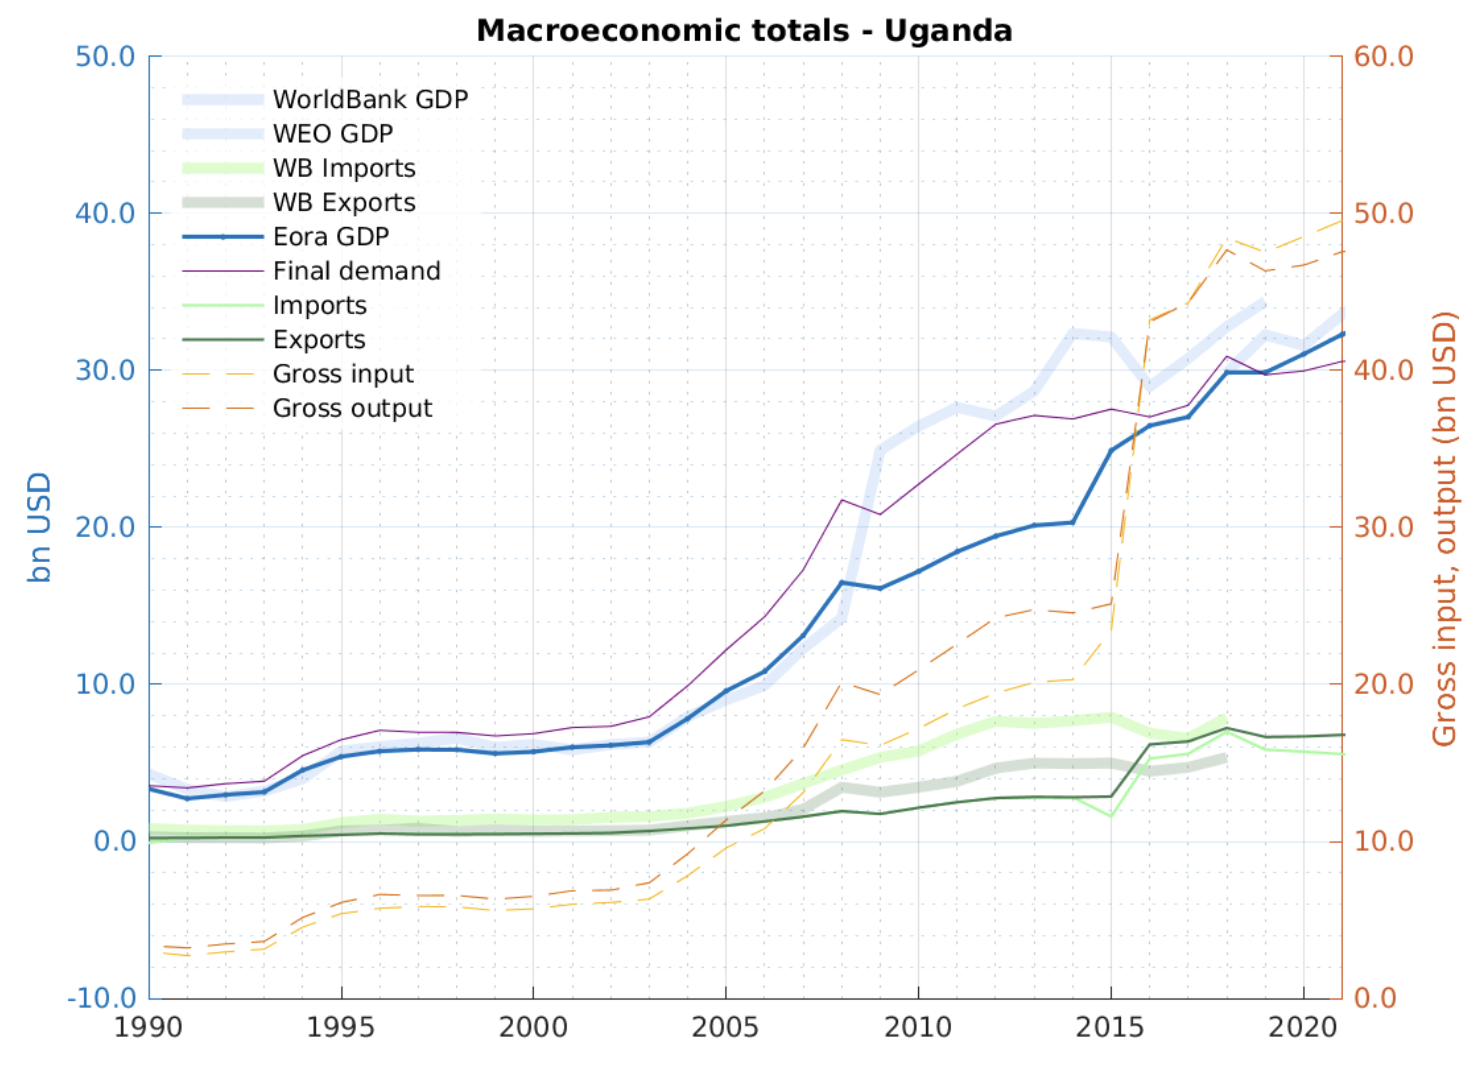
\includegraphics[width=0.5\textwidth, trim= {0 0 0 0}, clip]{"../Figures/DataQuality_UGA.png"} & 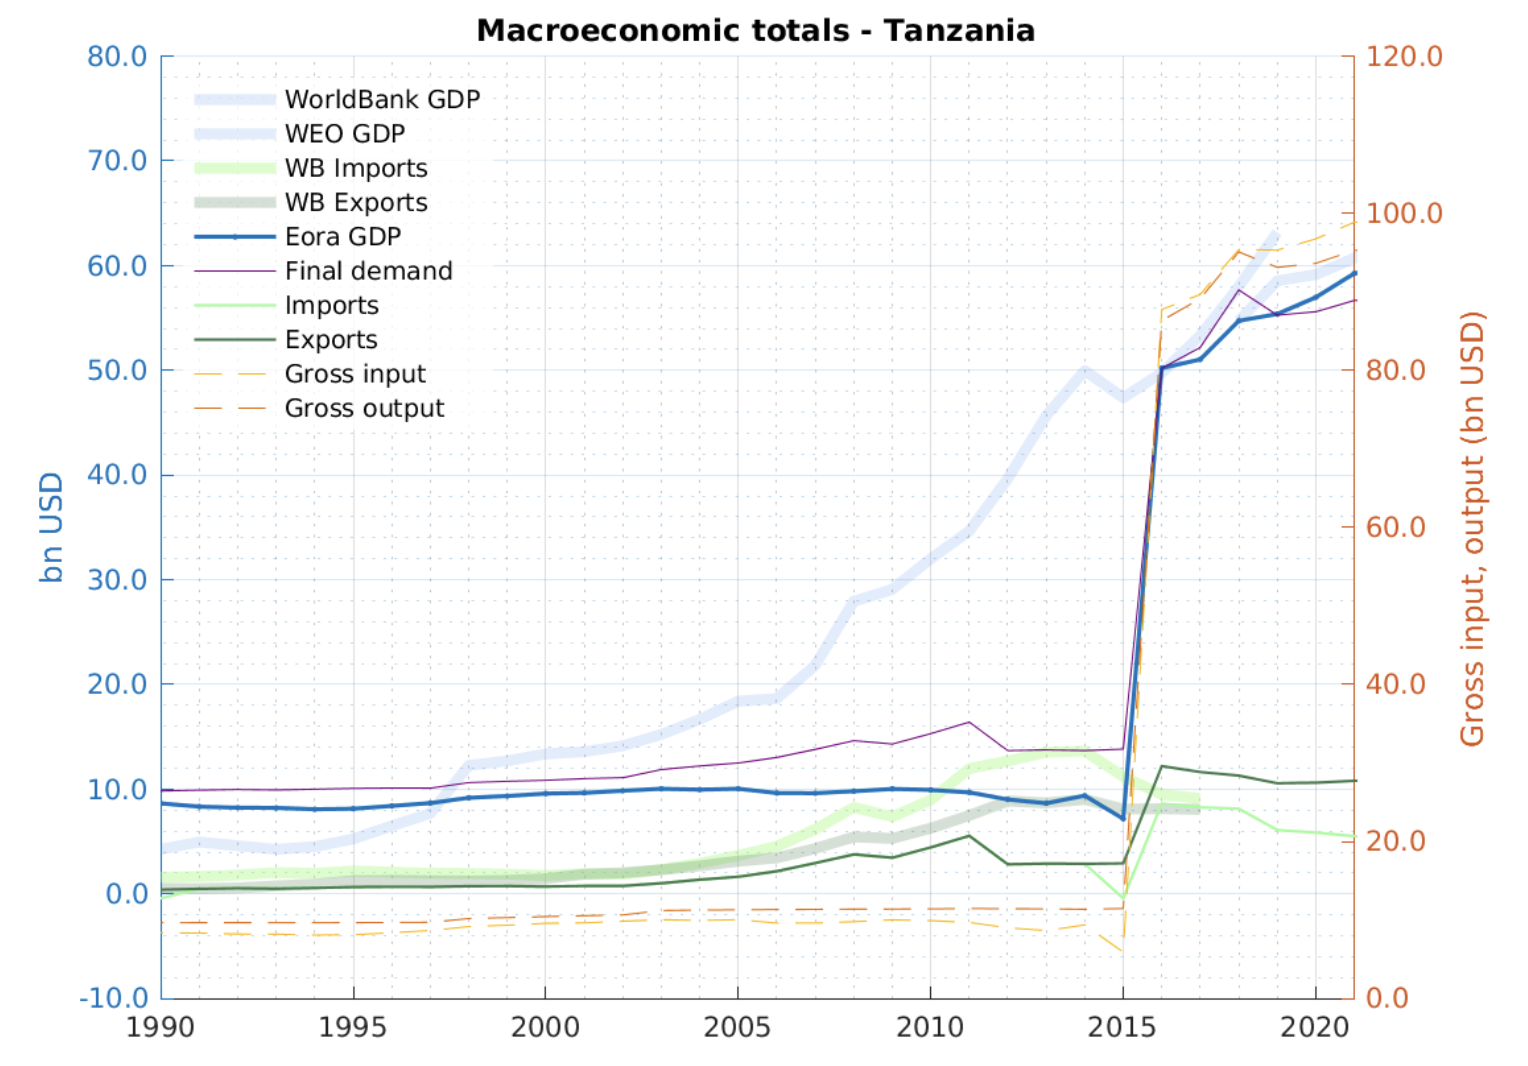
\includegraphics[width=0.52\textwidth, trim= {0 0 0 0}, clip]{"../Figures/DataQuality_TZA.png"} \\
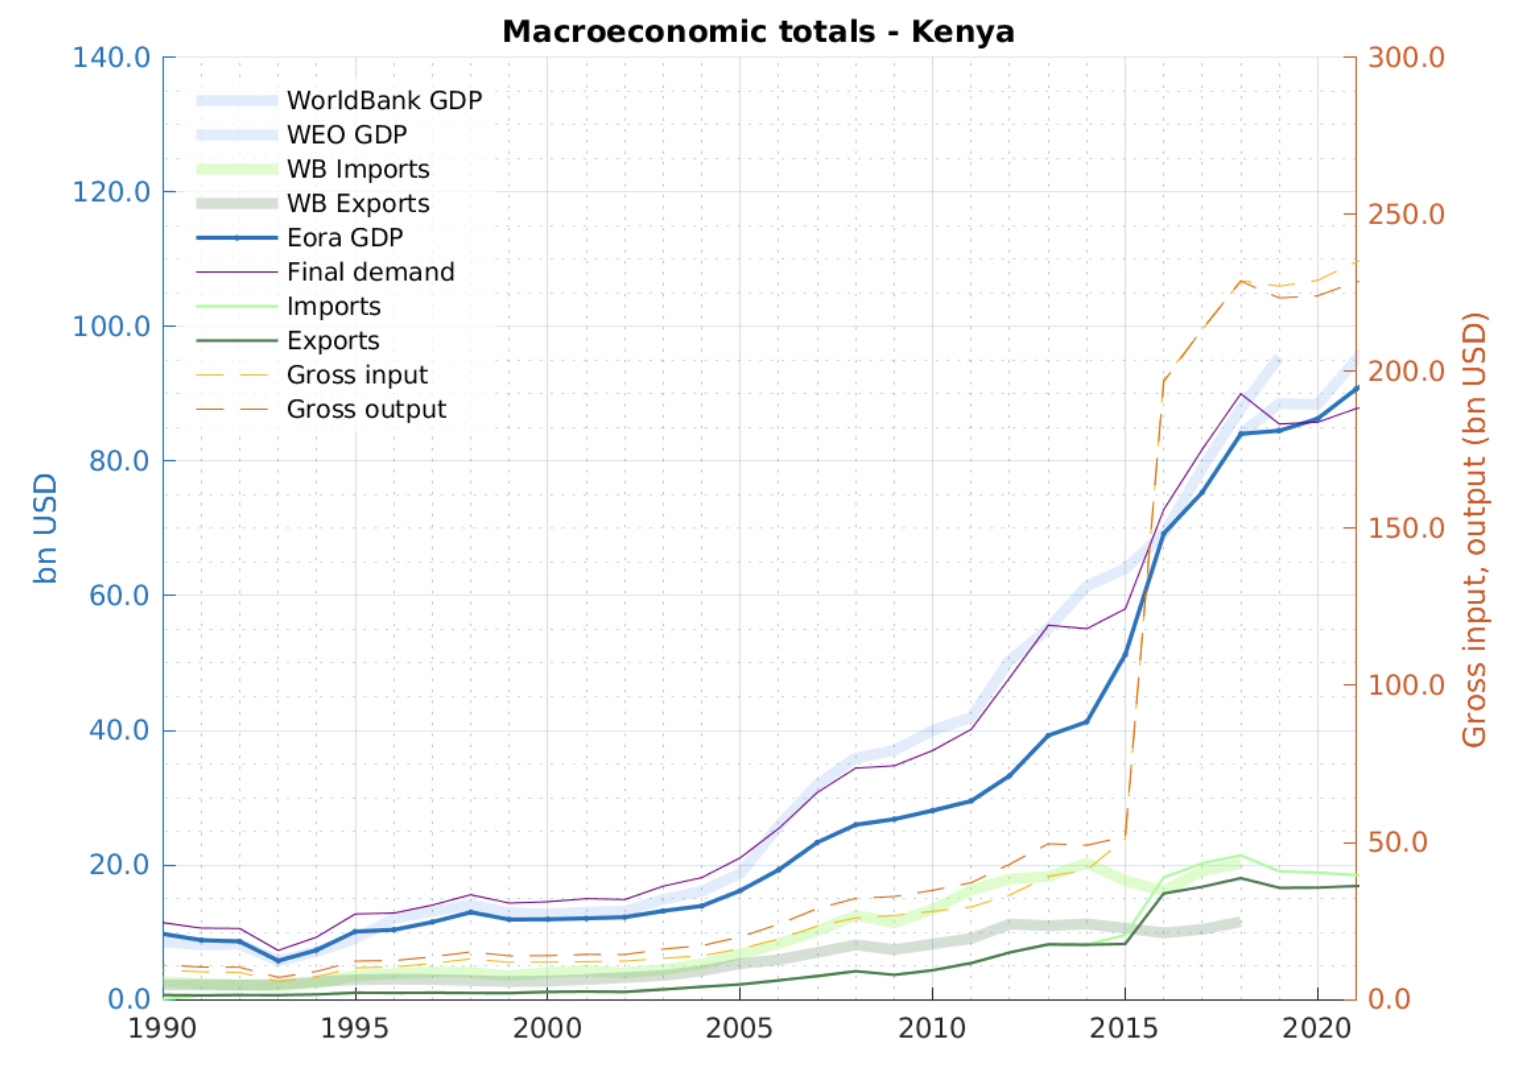
\includegraphics[width=0.5\textwidth, trim= {0 0 0 0}, clip]{"../Figures/DataQuality_KEN.png"} & 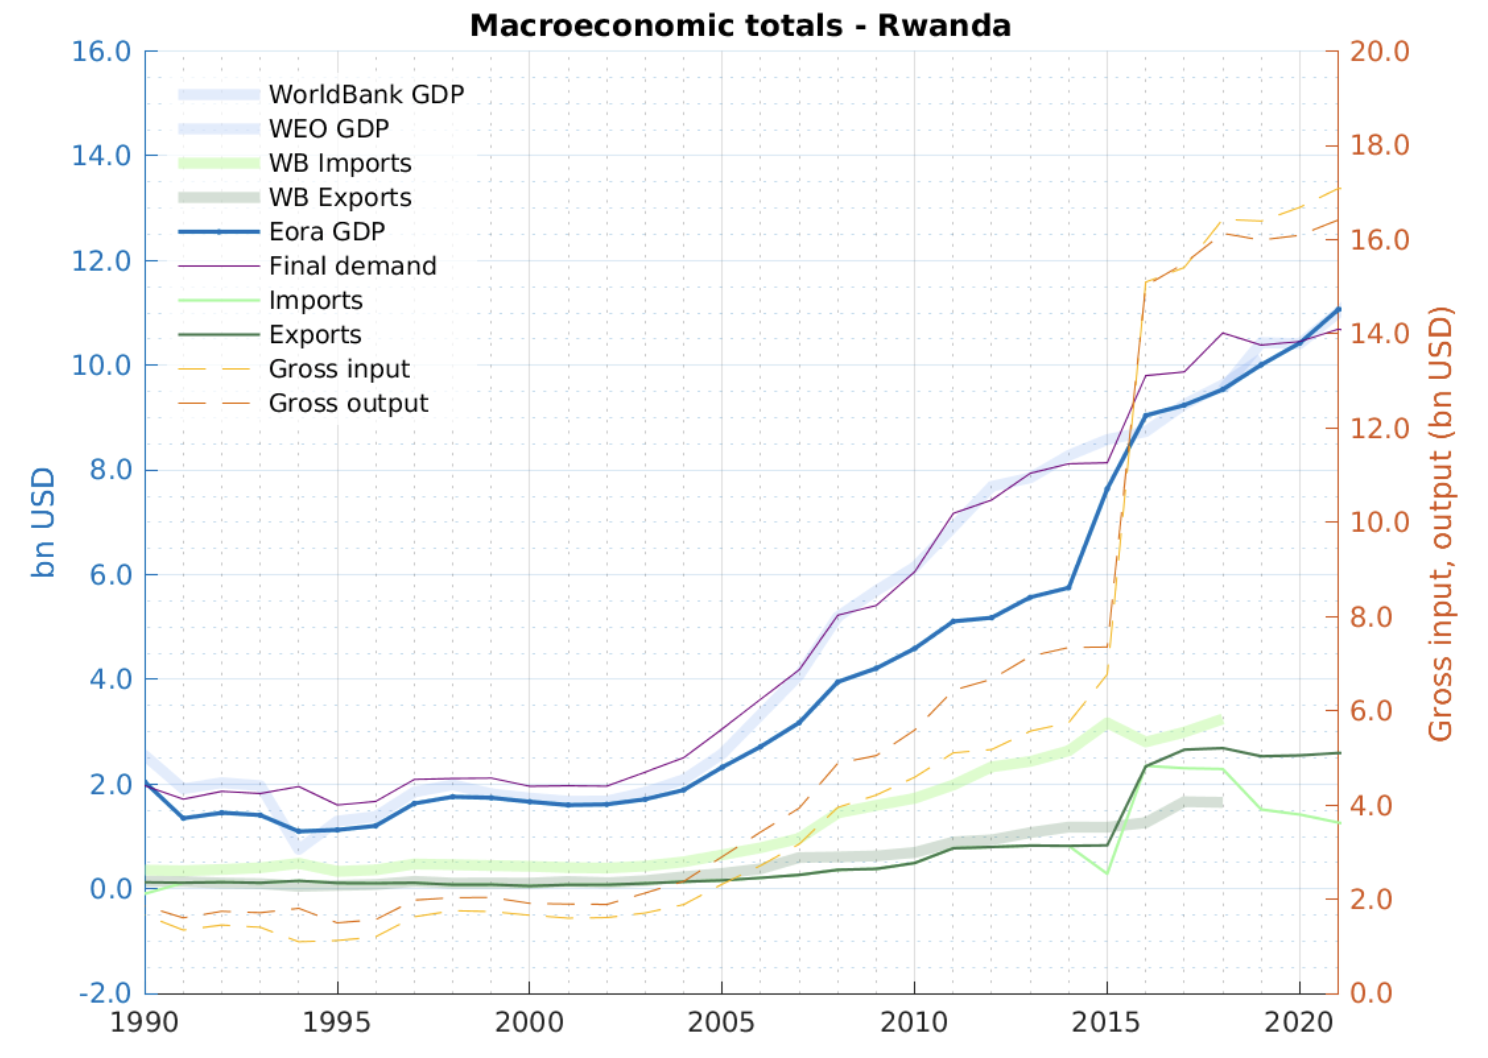
\includegraphics[width=0.5\textwidth, trim= {0 0 0 0}, clip]{"../Figures/DataQuality_RWA.png"} \\
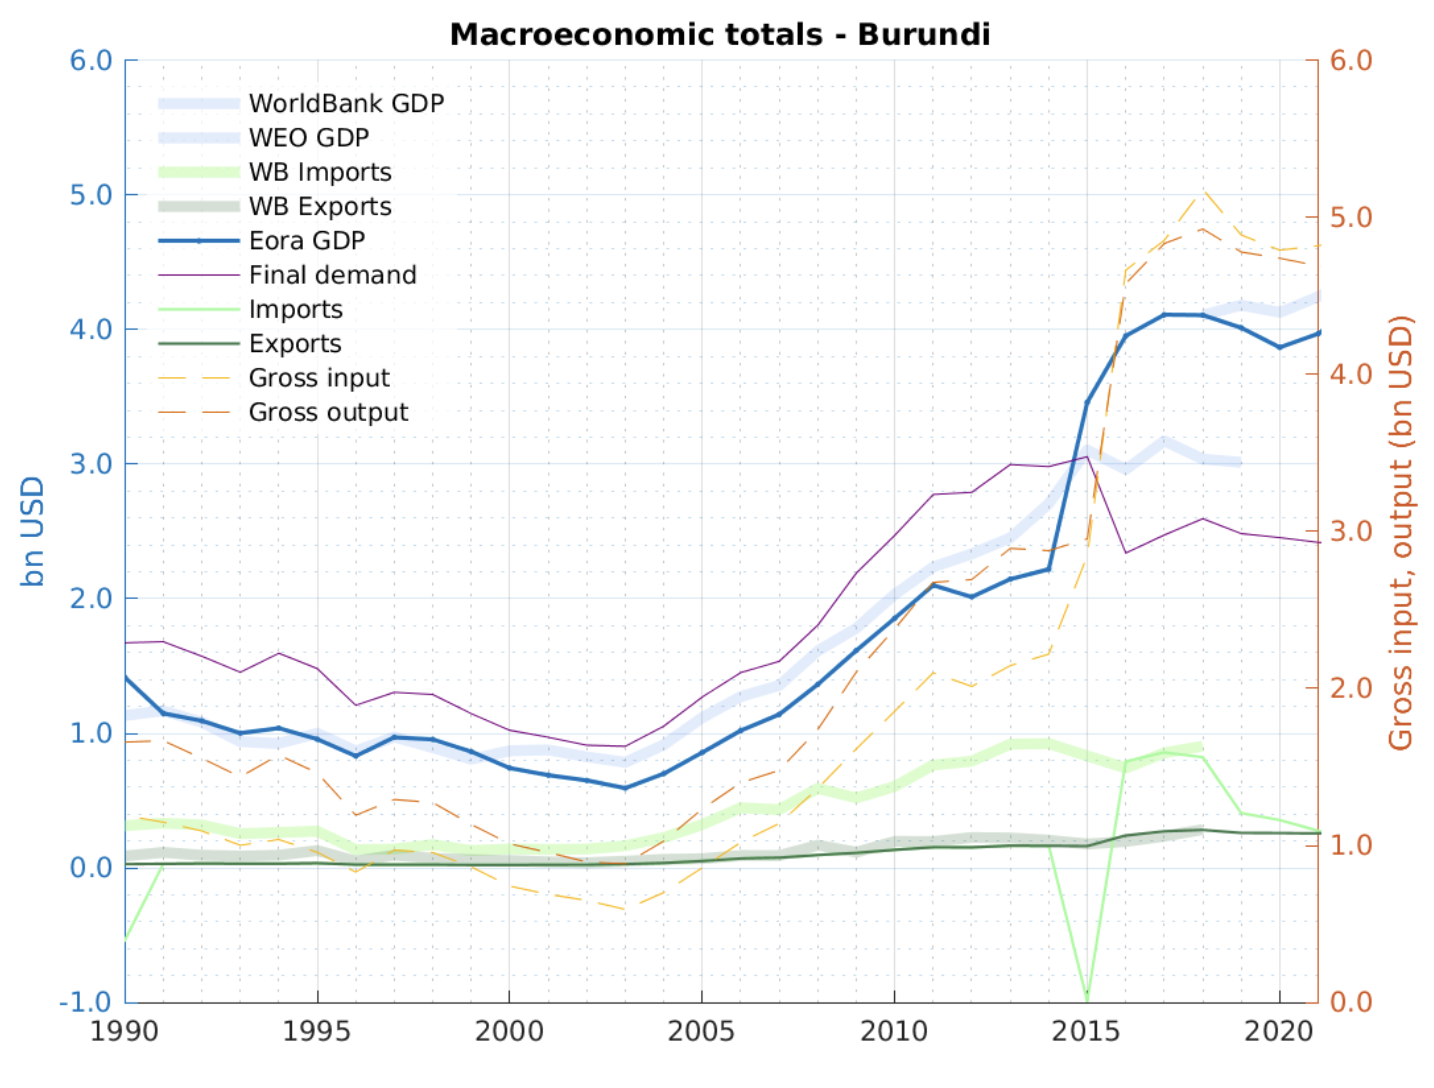
\includegraphics[width=0.5\textwidth, trim= {0 0 0 0}, clip]{"../Figures/DataQuality_BDI.png"} & \includegraphics[width=0.5\textwidth, trim= {0 0 0 0}, clip]{"../Figures/DataQuality_SSD.png"} \\
\end{tabular}
\end{figure}
\FloatBarrier


\subsection*{E. EORA 2021 Revision}
\setcounter{table}{0}
\renewcommand{\thetable}{E\arabic{table}}
\setcounter{figure}{0}
\renewcommand{\thefigure}{E\arabic{figure}}

The 2021 revision of EORA, incorporating updated administrative data from 2016 through 2018, and forecasts based on the World Economic Outlook through 2021, appears to better reflect macroeconomic totals for the EAC but also introduces major changes and structural breaks in GVC indicators, some of which appear highly unrealistic. 

\begin{figure}[h!]
\centering
\caption{\label{fig:EAC_GDP_sec_21}\textsc{EAC GDP by Sector: EORA 2021}}
\includegraphics[width=1\textwidth, trim= {0 0 0 0}, clip]{"../Figures/EAC_GDP_sector_21".pdf} %trim={<left> <lower> <right> <upper>}
\end{figure}
\FloatBarrier

Figure \ref{fig:exp21} shows gross exports in the extended database. The total export volumes appear closer to the true values (in 2018 according to World Bank Data Uganda exported \$3B, Tanzania \$4B, and Kenya \$6B in current prices), but the agricultural content of exports is overstated. Uganda for example had more than 40\% exports in mining in 2018. 

\begin{figure}[h!]
\centering
\caption{\label{fig:exp21}\textsc{EAC Gross Exports: EORA 2021}}
\includegraphics[width=1\textwidth, trim= {0 0 0 0}, clip]{"../Figures/exports_stacked_ts_21".pdf} %trim={<left> <lower> <right> <upper>}
\end{figure}
\FloatBarrier

Figure \ref{fig:outshares_ag_ts_21} shows the gross flows metrics. These also exhibit some large structural breaks, especially for Tanzania and Burundi, but no change to the overall story that Uganda and Kenya have significant export shares with the EAC, and Uganda and Rwanda have significant import shares with the EAC, while other countries' EAC engagement remains low. 

\begin{figure}[h!] % \vspace{-5mm}
\centering
\caption{\label{fig:outshares_ag_ts_21}\textsc{Decomposition of Output and Exports: EORA 2021}}
\includegraphics[width=1\textwidth, trim= {0 0 0 0}, clip]{"../Figures/output_shares_ag_ts_21".pdf} %trim={<left> <lower> <right> <upper>}
\vspace{-15mm}
\end{figure}
\FloatBarrier

Figure \ref{fig:VSag_ts_21} shows measures of forward and backward GVC integration with the updated EORA database. Compared to the pre-revision data, forward integration (E2R) is higher and backward integration (I2E) is lower. Notably, the high I2E in Tanzania seems to have been an artifact of the old data which vanishes in the updated data. The updated data however are also a source of problems. It is highly unrealistic that Burundi has a high level of backward integration at 50\% of exports being imported. 

\begin{figure}[h!] %\vspace{-5mm}
\centering
\caption{\label{fig:VSag_ts_21}\textsc{GVC Integration of EAC Members: Aggregate: EORA 2021}}
\includegraphics[width=1\textwidth, trim= {0 0 0 0}, clip]{"../Figures/VS_ag_ts_21".pdf} %trim={<left> <lower> <right> <upper>}
%\vspace{-10mm}
\end{figure}
\FloatBarrier

Figure \ref{fig:KWW_fill_ts_21} also shows the more detailed KWW decomposition with the KWW data, with similar results to Figure \ref{fig:VSag_ts_21}. The upstreamness and downstreamness ratios are computed from this data following equations \ref{eq:US} and \ref{eq:DS}, and displayed in Figure \ref{fig:UP_DOWN_ag_ts_21}. Figure \ref{fig:UP_DOWN_ag_ts_21} shows a structural break, but not really a trend reversal, in the upstreamness and downstreamness ratios. Thus the downstream shift observed up to 2015 is broadly continued in EORA 2021. \newline

Finally, Figures \ref{fig:NRCA_21} and \ref{fig:NRCA_EAC_21} show New Revealed Comparative Advantage (NRCA) in 2015 and 2021, in overall terms and relative to the EAC, respectively. Both estimates are still very close to the 2015 ones and suggest a continuation of the trend towards lower manufacturing competitiveness in all countries apart from Kenya already observed in the 2005-2015 period. \newline

In summary, EORA 2021 introduces a stark trend break and also distorts data for some countries and sectors, while giving an overall better representation of macroeconomic totals. It does however not change the fundamental conclusions about EAC integration into GVCs and RVCs reached by this paper using EORA 2015. Since such a stark trend break in the data is hard to vindicate, and EAC regional integration has not progressed much since the establishment of a common market in 2010, these findings also vindicate the choice to use EORA 2015.  


\begin{figure}[h!]
\centering
\caption{\label{fig:KWW_fill_ts_21}\textsc{KWW Decomposition of Gross Exports: EORA 2021}}
\includegraphics[width=1\textwidth, trim= {0 0 0 0}, clip]{"../Figures/KWW_fill_ts_21".pdf} %trim={<left> <lower> <right> <upper>}
\end{figure}
\FloatBarrier
 

\begin{figure}[h!] % \vspace{-0.4cm}
\centering
\caption{\label{fig:UP_DOWN_ag_ts_21}\textsc{Upstreamness and Downstreamness Ratios: EORA 2021}}
\includegraphics[width=1\textwidth, trim= {0 0 0 0}, clip]{"../Figures/UP_DOWN_ag_ts_21".pdf} %trim={<left> <lower> <right> <upper>}
% \vspace{-1cm}
\end{figure} 
\FloatBarrier 

\begin{figure}[h!]
\centering
\caption{\label{fig:NRCA_21}\textsc{New Revealed Comparative Advantage: EORA 2021}}
\includegraphics[width=1\textwidth, trim= {0 0 0 0}, clip]{"../Figures/NRCA_fl_21".pdf} %trim={<left> <lower> <right> <upper>}
\end{figure}
\FloatBarrier

\begin{figure}[h!]
\centering
\caption{\label{fig:NRCA_EAC_21}\textsc{NRCA Relative to EAC: EORA 2021}}
\includegraphics[width=1\textwidth, trim= {0 0 0 0}, clip]{"../Figures/NRCA_EAC_fl_21".pdf} %trim={<left> <lower> <right> <upper>}
\vspace{-1cm}
\end{figure}
\FloatBarrier



\end{document}
